\documentclass[11pt,a4paper]{exam}
\usepackage[utf8]{inputenc}
\usepackage{amsmath, amsthm, amssymb, amsfonts} %ams packages
\usepackage{graphicx, color} %grphics
\usepackage{enumitem} %personalized lists 
\usepackage[top=4cm, bottom=2cm, left=2cm, right=2cm, headsep = 3pt, footskip=2pt]{geometry} %pagelayout
\usepackage{multirow,multicol} %to use multirow on tables
\usepackage{tabularx}
\usepackage{array} %bmatrix and similar stuff
% \usepackage{hyperref}
\usepackage[slovene]{babel}

\usepackage{multicol}


%%%%%%%%%%%%%%%%%%%%%%%%%%%%%%%%%%%%%%%%%%%%%%%%%%%%%%%%%%%%%%%%%%%%%
%personalized commands to make latex look better (optional)
%%%%%%%%%%%%%%%%%%%%%%%%%%%%%%%%%%%%%%%%%%%%%%%%%%%%%%%%%%%%%%%%%%%%%%%%%%%
\renewcommand{\leq}{\leqslant} %menores y mayores iguales decentes
\renewcommand{\geq}{\geqslant}
\renewcommand{\subset}{\subseteq} 
\renewcommand{\supset}{\supseteq} 
\renewcommand{\subsetneq}{\varsubsetneq}
\renewcommand{\{}{\lbrace}
\renewcommand{\}}{\rbrace}
\newcommand{\sm}{\setminus} %setminus corto

%\renewcommand{\bar}{\overline}
%\renewcommand{\hat}{\widehat}

%%%%%%%%%%%%%%%%%%%%%%%%%%%%%%%%%%%%%%%%%%%%%%%%%%%%%%%%%%%%%%%%%%%%%}

%%%%%%%%%%%%%%%%%%%%%%%%%%%%%%%%%%%%%%%%%%%%%%%%%%%%%%%%%%%%%%%%%%%%%%%%%%%
%exam class commands
%%%%%%%%%%%%%%%%%%%%%%%%%%%%%%%%%%%%%%%%%%%%%%%%%%%%%%%%%%%%%%%%%%%%%%%%%%%
\pagestyle{head}
% \chead{ Matematična analiza 2024/2025 \\ Univerza v Ljubljani, Pedagoška fakulteta \\ Vaje 1 \\17. februar 2025} %self-explanatory
% \runningheader{}{ Abstraktna algebra 2024/2025 \\ Univerza v Ljubljani, Pedagoška fakulteta \\2. Kolokvij \\20. januar 2025}{} %self-explanatory
% \runningheader{}{}{}
% \footer{}{}{}
% \firstpagefooter{MATH 1190 3.0 M  }{Page \thepage\ of \numpages}{Copyright 2020 \textcopyright Antonio Montero}
% \firstpagefooter{}{}{}
% \runningfooter{MATH 1190 3.0 M }{Page \thepage\ of \numpages}{Copyright 2020 \textcopyright Antonio Montero}
% \firstpagefootrule 
% \runningfootrule

%%Solutions
\unframedsolutions
% \printanswers
\SolutionEmphasis{\itshape}


%Personalized commands
\pointpoints{točka}{točke}
% \gradetable[h][questions]
\addpoints
\hqword{Naloga}
% \vpgword{text}
\hpword{Točke}
% \hsword{}
% \hbpword{}
\htword{Skupaj}

% \pointsinrightmargin
% \extrawidth{-2cm}
\marginpointname{ \points}


\chqword{Naloga}
\chpgword{Stran}
\chpword{točke}
% \chbpword{Puntos extra}
% \chsword{Puntos obtenidos
\chtword{Skupaj}
%%%%%%%%%%%%%%%%%%%%%%%%%%%%%%%%%%%%%%%%%%%%%%%%%%%%%%%%%%%%%%%%%%%%%

% \graphicspath{{../img/}} %Uso: \graphicspath{{RelativePath}}

%%%%%%%%%%%%%%%%%%%%%%%%%%%%%%%%%%%%%%%%%%%%%%%%%%%%%%%%%%%%%%%%%%%%%
%Personalized commands

%Personalized commands

\usepackage{tabularx}
\newcolumntype{C}{>{\centering\arraybackslash}X}%
\newcolumntype{R}{>{\raggedleft\arraybackslash}X}%
\newcolumntype{L}{>{\raggedright\arraybackslash}X}%

\newcolumntype{\cc}[1]{>{\hsize=#1\hsize\raggedright\arraybackslash}X}%
\newcolumntype{\rr}[1]{>{\hsize=#1\hsize\raggedleft\arraybackslash}X}%
\newcolumntype{\ll}[1]{>{\hsize=#1\hsize\centering\arraybackslash}X}%

\newcommand{\TT}{\mathbf{T}}
\newcommand{\FF}{\mathbf{F}}

\DeclareMathOperator{\sh}{sh}
\DeclareMathOperator{\ch}{ch}
\let\th\relax
\DeclareMathOperator{\th}{th}
\DeclareMathOperator{\arsh}{arsh}
\DeclareMathOperator{\arch}{arch}
\DeclareMathOperator{\arth}{arth}
\DeclareMathOperator{\arctg}{arctg}

%%%%%%%%%%%%%%%%%%%%%%%%%%%%%%%%%%%%%%%%%%%%%%%%%%%%%%%%%%%%%%%%%%%%%
		\newif\ifmarking
% 		\markingtrue %comment to hide marking suggestions

		\newenvironment{marking}
		{\hrulefill
		 
		\textbf{Marking suggestions:} 
		\ttfamily }
		{\hrulefill }

\allowdisplaybreaks

% \renewcommand{\thepartno}{\roman{partno}}
\renewcommand{\partlabel}{(\textit{\thepartno})}
%%%%%%%%%%%%%%%%%%%%%%%%%%%%%%%%%%%%%%%%%%%%%%%%%%%%%%%%%%%%%%%%%%%%%

\begin{document}
\chead{Matematična analiza 2024/2025 \\ Univerza v Ljubljani, Pedagoška fakulteta \\ Vaje}
% \footer{}{}{}
\pagestyle{head}


% \paragraph{Ključni pojmi:} Motivacija odvode, definicija odvode, osnovne lastnosti, odvodi osnovnih funkcij. 
\section*{Vaje (20. in 21. februar 2025)}
\begin{questions}
	\question
	Po definiciji izračunajte odvode naslednjih funkcij v točki $a$.
	\begin{multicols}{2}
		\begin{parts}
			\part $f(x)=3$, $a=7$.
			% \part $f(x) = x^{3}$, $a=1$
			\part $f(x)= x^{2} +2x-1$, $a =2$.
			% \part $f(x) = \frac{3}{x^{3}}$, $a= -1$.
			\part $f(x)=\begin{cases} e^{-\frac{1}{x}}, & \text{če } x>0 \\ 0 & \text{če } x\leq 0\end{cases},$ $a=0$
			% \part $f(x) = -5x$, $a=1$.
			\part $f(x)=\frac{1}{x^2}$, $a=1$.
			\part $f(x)=\sqrt{x-4}$, $a=0$ in $a=1$.
			\part $f(x)=|x|$, $a=0$.
		\end{parts}
	\end{multicols}


 \question Po definiciji izračunajte odvode naslednjih funkcij:
	\begin{multicols}{2}
		\begin{parts}
			\part $f(x) = e^{2x+1}$,
			% \part $f(x)=\sqrt{2x}$
			\part $f(x) = x^3 + x^2$
			% \part $f(x) = \frac{1}{\sqrt{x+1}}$
			\part $f(x)=\sin(3x)$
			% \part $f(x) = \frac{1}{x - 1}$
			\part $f(x) = 3x + 2$
			% \part $f(x) = 9 - \frac{1}{2}x$
			\part $f(x) = 2x^2 + x - 1$
			% \part $f(x) = 1 - x^2$
			\part $f(x) = x^3 - 12x$
			% \part $f(x) = \frac{1}{x - 1}$
			\part $f(x) = \frac{1}{\sqrt{x}}$
		\end{parts}
	\end{multicols}

	\question Z uporabo znanih pravil za odvode, odvajajte naslednje funkcije:
	\begin{multicols}{2}
		\begin{parts}
			\part $f(x) = 2x^4 + 3x - x^{\frac{1}{2}} + x^{-2} -3$
			\part $f(x) = \frac{3}{x^2} + 2 \sqrt[3]{x \sqrt{x}} - \frac{3}{\sqrt{x}}$
			\part $f(x) = e^x \cos x$
			\part $f(x) = 2x^4 \tan(x)$
			\part $f(x) = (\sin x + 2^x) \log(x)$
			\part $f(x) = (x^2 + 2^x) \arcsin x$
			\part $f(x) = \frac{e^x}{\sin x}$
			\part $f(x) = \frac{\arctan x}{\ln x}$
			\part $f(x) = \frac{2e^x+1}{\sqrt[3]{x+\sin x}}$
			\part $f(x) = \frac{\ln(x)e^x}{\sin x}$
			\part $f(x) = \sin(3x + \frac{\pi}{3})$
			\part $f(x) = \sqrt[3]{x^2 - 2x}$
			\part $f(x) = \arcsin(1 + e^x)$
			\part $f(x) = e^{\sin x}$
			\part $f(x) = (1 + \ln(x))^{10} \cos(4x)$
			\part $f(x) = \frac{\arctan x}{\sqrt[3]{2x+1}+\sin(2x)}$
			\part $f(x) = \frac{e^{2x}+\arccos(x^2)}{\sqrt[5]{2x+1}}$
			\part $f(x) = \arctan(e^{2x+1} + \sqrt{2x+1})$
			\part $f(x) = \sqrt[5]{\cos(2\ln(x)) + 1}$
			\part $f(x) = (1 + x)^{\frac{1}{x}}$
			\part $f(x) = (1 + 2x)^{\sin^2(x)}$.
		\end{parts}
	\end{multicols}
\end{questions}

	% \section*{Seminar (predstavitve)}
% 	\subsection*{Hiperbolične funkcije}
% 		\emph{Hiperbolične kosinus}, \emph{sinus} in \emph{tangens} so definirane z naslednjimi predpisi:

% 			\begin{align*}
% 			\ch(x) = \frac{e^x + e^{-x}}{2}, &&
% 			\sh(x) = \frac{e^x - e^{-x}}{2}, &&
% 			\th(x)=\frac{\sh(x)}{\ch(x)}.
% 			\end{align*}


% Na območjih, kjer so hiperbolične funkcije injektivne, definiramo inverzne funkcije, \emph{area funkcije},  $\arch$, $\arch$ in $\arth$. 
% \begin{questions}

% 	\question Utemeljite, da je funkcija $\sh$ injektivna povsod $\mathbb{R}$,  njena zaloga vrednosti oziroma definicijsko območje $\arsh$ pa je $\mathcal{Z}_{\sh}=\mathcal{D}_{\arsh}=\mathbb{R}$. 
% 	Funkcija $\ch$ postane injektivna kot zožitev na $[0,\infty)$ z zalogo vrednosti $\mathcal{Z}_{\ch}= [1,\infty) = \mathcal{D}_{\arch}$, $\th$ pa je injektivna povsod na $\mathbb{R}$ z zalogo vrednosti $\mathcal{Z}_{\th}= (-1,1) = \mathcal{D}_{\arth}$. 
	
% 	\textbf{Ne pozabite}: Če je $f: D \subset \mathbb{R} \to \mathbb{R}$ funkcija, množico $D$ imenujemo \emph{definicijsko območje}, pa množico $\mathcal{Z}_{f}=f(D)= \{f(x): x \in D\}$ imenujemo \emph{zaloga vrednosti} funkcije $f$. V kolikor je funkcija $f$ podana samo s predpisom za domeno običajno vzamemo največjo podmnožico $\mathcal{D}_f \subset \mathbb{R}$, na kateri je ta predpis smisel. 
	
% 	\question Izpelji naslednji zvezi med hiperboličnimi funkcijami:
% 	    \begin{align*}
% 	    \ch^2 (x) - \sh^2 (x) = 1, &&\th^2 (x) = 1 - \frac{1}{\ch^{2}(x)}.
% 	    \end{align*}
	
	
% 	  Pokažite tudi, da lahko area funkcije izrazimo z ostalimi elementarnimi funcijami na naslednji način:
% 	    \begin{alignat*}{2}
% 	    \arsh(x) &= \ln (x + \sqrt{x^{2}+1}), &\quad  x &\in \mathbb{R}; \\ 
% 	    \arch(x) &= \ln (x + \sqrt{x^{2}-1}), &  x &\geq 1; \\
% 	    \arth(x) &= \frac{1}{2}\ln \left( \frac{1+x}{1-x}\right),& x &\in (-1,1).
% 	    \end{alignat*}
% 	\question Dokažite, da so odvodi hiperboličnih in njihovih inverznih funkcij enaki:
	
% 	    \begin{align*}
% 	    \sh'(x)&=\ch(x) &\qquad \arsh'(x)&= \frac{1}{\sqrt{x^{2}+1}} \\
% 	    \ch'(x)&=\sh(x) &\qquad \arch'(x)&= \frac{1}{\sqrt{x^{2}-1}} \\
% 	    \th'(x)&=\frac{1}{\ch^{2}(x)} &\qquad \arth'(x)&= \frac{1}{1-x^{2}} \\
% 	    \end{align*}
% \end{questions}
% \pagestyle{empty}
% \clearpage


%%%%%%%%%%%%%%%%%%%%%%%%%%%%%%%%%%%%%%%%%%%%%%%%%%%%%%%


% \chead{Matematična analiza 2024/2025 \\ Univerza v Ljubljani, Pedagoška fakulteta \\ Vaje 2 \\27. in 28. februar 2025}
% \pagestyle{head}
% \paragraph{Ključni pojmi:} Tangenta/normala, odvodi implicitnih funkcij, ekstreme točke.
\section*{Vaje (27. in 28. februar 2025)}
\begin{questions}
	\question	
	Dana naj bo funkcija $f(x) = x^{3} - 11 x + 7$.
	\begin{parts}
    \part Zapišite enačbo tangente in normale na graf funkcije $f$ v točki $(3,1)$.
    \part Določi tangente na graf funkcije $f$ s koeficientom $-8$. Poiščite vse tangente na graf funkcije $f$, ki sekajo abscisno os pod kotom $\frac{\pi}{4}$.
	\end{parts}
	
	\question
	Poiščite vse tangente na graf funkcije $f(x) = x^{3} -6x^{2}+10x-4$, ki z abscisno osjo oklepajo kot $\frac{\pi}{4}$.

	\question Poiščite enačbo titst tangente na graph funkcije $f(x)= 2+x-x^{2}$, ki je vzporedna premici $y=\sqrt{3} - 3x$.

	\question
	Dana je funkcija $g(x) = \frac{x^{3}}{3}$.
	\begin{parts}
	\part Določite tangento in normalno na graf funkcije $g$ v točki $(-3,-9)$. 
	\part Poiščite vse tangente na graf funkcije $g$, ki so vzporedne premici $y=4x-2$, ter tudi vse tangente, ki sekajo $x$-os pod kotom $\frac{\pi}{4}$.
	\part Določite koeficient premice $y=kx-18$, da bo ta tangenta na graf funkcije $g$.
	\end{parts}

	\question
	Poiščite kot med krivuljama z enačbama $y + x^{2}+3x -2$ in $y = 2x^{2}-6$, t.j. kot med ustreznima tangentama na krivulji v presečni točki.

	\question Za naslednje funkcije določite maksimum in minimum na danih intervalih. Določite tudi intervale naraščanja in padanja danih funkcij na $\mathbb{R}$. Poiščite in klasificiraj stacionarne točke.
	\begin{parts}
    \part $f(x) = x^{4}-6x^{2}+8x +4$ na $\left[-\frac{3}{2},2\right]$;
    \part $f(x) = x^{2} e^{x}$ na $\left[-3,1\right]$;
    \part $f(x) = x - \cos(2x)$  na $\left[0, \pi\right]$;
    \part $f(x)=x^3-3x+3$ na $\left[-\frac{3}{2} ,3\right]$;
    \part $f(x) = x^4 - 6x^2 + 8x + 4$ na $\left[ -\frac{5}{2}, 2 \right]$;
    \part $f(x) = x^2 e^x$ na $[-3,1]$;
	\end{parts}

	\question Zapišite število $2025$ ko vsoto dveh nenegativnih realnih števil, da bo njun produkt največji možen.

	\question
 	Krogli s polmeron $R$ včrtaj pokončni stožec z največjo možno prostornino. Zapišite dobljeno maksimalno prostornino.

	\question
	Babica Jožica želi imeti ograjen zelenjavni vrt pravakotne oblike s površino $10 \ m^2$, ki bo tik ob eni izmed seten njene hiše. (Ograditi je traba le tri stranice.) Kakšnih dimenzij naj bo vrt, da bo zanj potrebno najmanj ograje?

	\question
	Babica Francka želi imeti zelenjavni vrt pravokotne oblike, ki bo tik ob eni izmed sten njene hiše. (Ograditi je traba le tri stranice.) Na voljo ima $10$ metrov ograje. Kakšnih dimenzij naj bo vrt, da bo njegova površina največja?

\end{questions}



% \section*{Seminar (predstavitve)}
	\begin{questions}
		\question Naj bodo $f$, $g$ in $h$ funkcije.
		\begin{parts}
			\part Predpostavimo, da velja \( f(a) = g(a) = h(a) \), da za vsak \( x \) velja \( f(x) \leq g(x) \leq h(x) \) in da je \( f'(a) = h'(a) \). 
			Dokažite, da je \( g \) odvedljiva v \( a \) in da velja \( f'(a) = g'(a) = h'(a) \). 
			\textbf{Nasvet}: začnite z definicijo \( g'(a) \).
			\part Dokažite, da sklep ne velja, če izpustimo predpostavko \( f(a) = g(a) = h(a) \).  
			\part 
			Naj bo $f(x)$ funkcija definirana kot
			\[
				f(x)= \begin{cases} x^{2} & \text{če je } x \in \mathbb{Q}; \\ 0 &\text{če je } x \in \mathbb{R} \setminus \mathbb{Q}. \end{cases}
				\]
				Dokažite, da je $f$ odvedljiva v $0$. \textbf{Nasvet}: ni tako težko. Uporabite lahko prejšnjo vajo.
			\end{parts}
				
		\question
		Funkcija $f$ je \emph{soda funkcija}, če za vsak $x$, za katerega je funkcija definirana, velja: $f(x) = f(-x)$. Funkcija $f$ je \emph{liha funkcija}, če za vsak $x$, za katerega je funkcija definirana, velja: $f(-x) = -f(x)$.
		\begin{parts}
			\part Razložite, kaj pomeni, da je funkcija $f$ soda (oz. liha) glede na graf funkcije $f$.
			\part Poiščite primer sode funkcije in primer lihe funkcije.
			\part Dokažite, da če je $f$ soda funkcija, velja $f'(x) = -f'(-x)$; narišite sliko. Dokažite, da če je $f$ liha funkcija, potem velja \( f'(x) = f'(-x) \). Prav tako narišite skico.
		\end{parts}
		
		\question Naj bosta $f$ in $g$ funkciji. 
		\begin{parts}
			\part Če je $f+g$ odvedljiva v točki $a$, ali sta $f$ in $g$ nujno odvedljivi v $a$? 
			\part Če sta $f \cdot g$ in $f$ odvedljiva v $a$, pod katerimi pogoji za $f$ sledi, da je tudi $g$ odvedljiva v $a$?
			\part Dokažite, da če je $f$ odvedljiva v točki $a$, potem je tudi $|f|$ odvedljiva v $a$, kadar $f(a) \neq 0$. 
			\part Podajte protiprimer prejšnje trditve, če je $f(a) = 0$. 
			\part Dokažite, da če sta $f$ in $g$ odvedljivi v $a$, potem sta tudi funkciji $\max(f,g)$ in $\min(f,g)$, definirani s predpisoma 
			\begin{align*}
				\max(f,g)(x) &= \max\{f(x),g(x)\} \text{ in }\\
				\min(f,g)(x) &= \min\{f(x),g(x)\},
			\end{align*}
			odvedljivi v $a$, kadar $f(a) \neq g(a)$.
			\part Podajte protiprimer prejšnje trditve, če je $f(a) = g(a)$.
		\end{parts}
	\end{questions}
\pagestyle{empty}
\clearpage


%%%%%%%%%%%%%%%%%%%%%%%%%%%%%%%%%%%%%%%%%%%%%%%%%%%%%%%


% \chead{Matematična analiza 2024/2025 \\ Univerza v Ljubljani, Pedagoška fakulteta \\ Vaje 3 \\6. in 7. marec 2025}
% \pagestyle{head}
% \paragraph{Ključni pojmi:} ekstreme točke, Rollov izrek, Lagrangeev izrek.
\section*{Vaje (6. in 7. marec 2025)}
\begin{questions}

	\question Dana je funkcija $f(x) = e^{x}$.
		\begin{parts}
			\part Zapošite enačbo tangente na graf funkcije $f$ v točki $x=1$.
			\part Dokažite, da za vsako realno število $x$ velja $e^{x} \geq e x$.
		\end{parts} 

	 \question Mojster Miha želi zgraditi silos za žito v obliki valja s sferno kupolo. Cena materiala za kupolo je dvakrat večja od cene materiala za valjasti del silosa. Kakšnih dimenzij naj bo silos za $1000 \ { m}^3$ žita, da bo njegova izgradnja najcenejša?


			\question Izdelati želimo lonec brez pokrova v obliki valja za $10$ litrov juhe. Kakšne morajo biti dimenzije, da se porabi čim manj materiala? (Debelino lonca lahko zanemarimo.)

			\question Ali lahko uporabite Rollov izrek za funkcijo $f(x) = x^{7}-2x^2-x+4$ na intervalu $[-1,1]$. Če je odgovor pritrdilen, ga zapišite.

			\question Dana je zvezna funkcija $f: [a,b] \to \mathbb{R}$, ki je odvedljiva na intervalu $(a,b)$ in osemkrat zavzame isto vrednost (npr. 2). Z uporabo Rollovega izreka dokažite, da ima potem odvod funkcije $f'$ na intervalu $(a,b)$ vsaj se dem ničel. Ali lahko rezultat posplošite na funkcijo z $n$ ničlami, t.j. ugotovite in utemeljite, najmanj koliko ničel ima odvod $g'$ če ima $g$ natanko $n$ ničel?

			\question 
				\begin{parts}
					\part Zapišite trditev Lagrangeevega izreka za funkcijo $f(x) = (1+x)^{\alpha}$ na intervalu $[0,z]$, kjer sta $\alpha > 1$ in $z >0$ dve konstanti.
							\part S pomočjo zgoraj zapizanega pokažite posplošeno Bernoullijevo neenakost:
							\begin{align*} (1+z)^{\alpha} \geq 1+\alpha z && z > 0, \alpha > 1. \end{align*}
				\end{parts}
			
			\question Dokažite, da za vsako odvedljivo funkcijo $f \colon (a,b) \to \mathbb{R}$ z vsaj dvema fiksnima točkama obstaja taka točka $\xi \in (a,b)$, za katero je $f'(\xi) = 1$.

			\question Dokažite, da velja:
				\begin{parts}
					\part $|\arctan(x) - \arctan(y)| \leq |x-y|$, za $x,y \in \mathbb{R}$.
					\part $|\sin(2x) - \sin(2y)| \leq 2|x-y|$, za $x,y \in \mathbb{R}$.
					\part Za vsako zvezno odveljivo funkcijo $f\colon [a,b] \to \mathbb{R}$ obstaja konstanta $C > 0$, da velja  \[ |f(x) - f(y)| \leq C|x-y|, \text{ za } x,y \in [a,b]. \]
				\end{parts}


\end{questions}
% \section*{Seminar (predstavitve)}
% 	\begin{questions}
% 		\question Dani $f \colon [a,b] \to \mathbb{R}$  in $g \colon [a,b] \to \mathbb{R}$  zvezni  funkciji na $[a,b]$ in odvedljivi na $(a,b)$.
% 			\begin{parts}
% 				\part Dokažite, da če je $f'(x) = 0$ za vsak $x \in (a,b)$, potem je $f$ konstantna funkcija.
% 				\part Če velja da $f'(x) = g'(x)$ za vsak $x \in (a,b)$, potem obstaja $k \in \mathbb{R}$, da velja $f(x) = g(x) + k$ za vsak $x \in (a,b)$.
% 				\part Predpostavimo, da velja $|f(x) - f(y)| \leq (x - y)^n$ za nekaj $n > 1$.  Dokažite, da je $f$ konstantna.
% 				\part Predpostavimo, da je $f'(x) > g'(x)$ za vsak $x$ in da za nekaj $c \in  (a, b)$  velja $f(c) = g(c).$ Dokažite, da $f(x) > g(x)$ za $x > c$ in $f(x) < g(x)$ za $x < c$.
% 				\part S primerom pokažite, da prejšnja trditev ne drži brez predpostavke $f(c) = g(c)$.
% 			\end{parts}

% 			\question Dana je funkcija $f(x) = \ln(x)$.
% 				\begin{parts}
% 				\part Zapožite trditev Lagrangeevega izreka za funkcijo $f$ na intervalu $[a, a+1]$, kjer $a > 0$. S pomožjio dobljenega nato dokažite neenakost:
% 					\[
% 						\frac{1}{1+a} < \ln \left( 1 + \frac{1}{a} \right) < \frac{1}{a}, \qquad a>0.
% 					\]
% 					\part S pomočjo zgoraj dokazane neenakosti dokažite, da za delne vsote harmonične vrste velja:
% 					\[
% 						\ln(n) + 1 \geq 1 + \frac{1}{2}+ \frac{1}{3} + \cdots + \frac{1}{n} > \ln(n+1), \qquad n \in \mathbb{N}.
% 					\]
% 				\end{parts}

	
		
% 	\end{questions}
% \pagestyle{empty}
% \clearpage


%%%%%%%%%%%%%%%%%%%%%%%%%%%%%%%%%%%%%%%%%%%%%%%%%%%%%%%


% \chead{Matematična analiza 2024/2025 \\ Univerza v Ljubljani, Pedagoška fakulteta \\ Vaje 4 \\13. in 14. marec 2025}
% \pagestyle{head}
% \paragraph{Ključni pojmi}: Lagrangeev izrek, L'Hopitalovo pravilo, grafi funkcij, parametrične in polarne krivulje.	
\section*{Vaje (13. in 14. marec 2025)}
\begin{questions}
	\question Dokažite, da velja:
		\begin{parts}
			\part $|\arctan(x) - \arctan(y)| \leq |x-y|$, za $x,y \in \mathbb{R}$.
			\part $|\sin(2x) - \sin(2y)| \leq 2|x-y|$, za $x,y \in \mathbb{R}$.
			\part Za vsako zvezno odveljivo funkcijo $f\colon [a,b] \to \mathbb{R}$ obstaja konstanta $C > 0$, da velja  \[ |f(x) - f(y)| \leq C|x-y|, \text{ za } x,y \in [a,b]. \]
		\end{parts}

		\question S pomočjo L'Hopitalovega pravila ali kako drugače izračunajte naslednje limite:
		\begin{multicols}{2}
			\begin{parts}
				\part $\lim_{x\to\infty} \frac{2x^3 + x - 2}{e^x}$;
				% \part $\lim_{x\to 0} \frac{\tan(x)}{x}$;
				% \part $\lim_{x \to \infty} \frac{\ln(x)}{x}$;
				\part $\lim_{x \to \infty} \frac{\ln(x)}{\sqrt[3]{x}}$;
				% \part $\lim_{x \to 0} \frac{\ln(1 + x^2)}{\sin(2x)}$;
				% \part $\lim_{x \to \infty} \frac{\ln(\ln x)}{\ln x}$
				% \part $\lim_{x \to 3} \frac{\arcsin(x - 3)}{x^2 - 3x}$;
				% \part $\lim_{x \to 0} \frac{\ln(1 + x) - x}{x \sin(x)}$;
				% \part $\lim_{x \to 0} \frac{\ln(1 + x) - x}{(\sin x)^2}$
				% \part $\lim_{x\to 0} \frac{\operatorname{arctg}(2x)}{4x}$; 
				% \part $\lim_{x \to 0} \frac{x - \arctg(2x)}{x - \sin(3x)}$;
				\part $\lim_{x \to 0} \arcsin(2x) \cot(3x)$;
				% \part $\lim_{x \to \infty} x \left(e^{\frac{1}{x}} - 1\right)$;
				\part $\lim_{x\to 0} x (\ln(x))^3$ ; 
				\part $\lim_{x \to 1} \left(\frac{x}{x - 1} - \frac{1}{\ln(x)}\right)$;
				% \part $\lim_{x \to 0} \left(\frac{1}{x^2} - \frac{\cot(x)}{x} \right)$;
				% \part $\lim_{x \to 0^+} x^x$;
				% \part $\lim_{x\to 0} \frac{x - \operatorname{arctg}(x)}{x^3}$; 
				\part $\lim_{x\to\infty} (1 + x)^{\frac{1}{x}}$.
			\end{parts}
		\end{multicols}
	
		\question Kje se nahaja napaka v naslednji uporabi L'Hopitalovega pravila?:
		Naj bosta $f(x) = x^3 + x - 2$ in $g(x)=x^2 - 3x + 2$.
		%
		%
		\begin{align*}
			\lim_{x\to 1} \frac{x^3 + x - 2}{x^2 - 3x + 2} &= \lim_{x\to 1} \frac{f(x)}{g(x)}\\
			&= \lim_{x\to 1} \frac{f'(x)}{g'(x)} && \text{(L'Hopitalovo pravilo)} \\
			&= \lim_{x\to 1} \frac{(f'(x))'}{(g'(x))'} && \text{(L'Hopitalovo pravilo)} \\
			&=\lim_{x\to 1} \frac{(3x^2 + 1)'}{(2x - 3)'}\\
			&=\lim_{x\to 1} \frac{6x}{2} \\
			&=3
		\end{align*}
		%
		\textbf{Nasvet}: Pravilna vrednost limite je 4.


		\question Dane so funkcije
\begin{multicols}{2}
\begin{itemize}
	\item $f(x) = 3x^4 + 8x^3 + 6x^2 - 5$;
	% \item $f(x) = \sqrt{x}(2 - x)$;
	% \item $f(x) = x\sqrt{1 - x^2}$;
	% \part $f(x) = \frac{\sqrt{2x + 4}}{x + 4}$;
	\item $f(x) = \frac{x - 1}{\sqrt{x^3}}$
	% \item $f(x) = x^2 e^{-x} + 1$
	% \item $g(x) = (x^2 - 2x - 1)e^{\frac{1}{2}x}$;
	% \item $k(x) = \frac{e^x}{x^2 - 3}$;
	\item $f(x) = x e^{1 - x^2}$;
	% \item $f(x) = \ln(2x - 1) - 3x$;
	% \item $f(x) = \frac{1}{x} + 2\ln(3x)$;
	% \item $f(x) = \frac{x}{\ln(x)}$;
	% \item $g(x) = \frac{2 - 5\ln(x)}{x^2}$;
	\item $f(x) = x^2 (\ln(x))^2$
	% \item $g(x) = \frac{2}{3 - x} - \arctg(x)$;
	% \item $g(x) = \frac{1}{x} + 2\arctg(x)$;
	% \item $f(x) = \arctg(2x) - \arctg\left(\frac{1}{x}\right)$;
	% \item $h(x) = e^{\sin(x)}$.
\end{itemize}
\end{multicols}
\begin{parts}
	\part Danim funkcijam določite defininicijsko območje, ničle, pole, asimptote in raziščite obnaǎnje na robu definiciskega območja.
 \part Poiščite intervale naraščanja in padanja, lokalne ekstreme, ter zalogo vrednosti danih funkcij.
 \part Določite intervale konveksnosti in konkavnosti, ter prevoje. Če ne gre v splošnem, potem poiščite vsaj kakšno točko, v okolici katere je dana funkcija konveksna oziroma konkavna.
\part Čimbolj natančno skiciraj graf funkcije.
\end{parts}

\question V implicitni in parametrični obliko so podane naslednje krivulje:
\begin{itemize}
    \item $ x(t) = 4\cos(t), \quad y(t) = 3\sin(t), \quad t \in \mathbb{R}$, (elipsa);
    % \item $ x(t) = \pm 4\cosh(t), \quad y(t) = 3\sinh(t), \quad t \in \mathbb{R}$, (hiperbola);
    \item $ x^{\frac{2}{3}} + y^{\frac{2}{3}} = 1$, (asteroida). \textbf{Nasvet}: Parametriziraj z $ x(t) = \cos^3(t), \quad y(t) = \sin^3(t), \quad t \in [0,2\pi] $;
    % \item $ x(t) = \sin(2t), \quad y(t) = \sin(t), \quad t \in \mathbb{R}$;
    % \item $ x(t) = t^2 - 1, \quad y(t) = t(t^2 - 1), \quad t \in \mathbb{R}$;
    % \item $ x(t) = a(t - \sin t), \quad y(t) = a(1 - \cos t), \quad t \in \mathbb{R}, \quad a > 0 $, (cikloda);
    % \item $ x^3 - 3axy + y^3 = 0, \quad a > 0$, (Descartesov list). \textbf{Nasvet}: Vpelji parameter $ t = \frac{x}{y} $;
    % \item $ x = \cos(at), \quad y = \sin(at), \quad z = bt, \quad t \in \mathbb{R}, $ (vijačnica).
\end{itemize}
\begin{parts}
	\part Čimbolj natančno narišite krivulje. Nasvet: Skicirajte grafa $x(t)$ in $y(t)$, ter poskusite določiti ekstremne točke, t.j. rešite tenačbi $\dot{x} =0$ in $\dot{y}=0$.
	\part Izračunajte naklon krivulje oziroma $y'$. Izberite si neko točko na krivulji in določite tangento na dano krivuljo v tej točki, če obstaja.
\end{parts}

V implicitni ali polarni obliki so podane naslednje krivulje:
\begin{itemize}
    % \item $ r(\varphi) = \frac{a}{\varphi}, \quad \varphi \in \mathbb{R}^+$, (hiperbolična spirala).
    % \item $r(\varphi) = e^{a\varphi}$, (logaritemska spirala).
    \item $r(\varphi) = \cos(3\varphi), \quad \varphi \in \left[-\frac{\pi}{6}, \frac{\pi}{6} \right] \cup \left[\frac{\pi}{2}, \frac{5\pi}{6} \right] \cup \left[\frac{7\pi}{6}, \frac{9\pi}{6} \right]$.
    \item $r(\varphi) = a(1 + \cos(\varphi)), \quad \varphi \in [-\pi, \pi] $, (kardioida).
    % \item $(x^2 + y^2) = 2a^2(x^2 - y^2), \quad a > 0$, (lemniskata). \textvf{Nasvet}: Vpelji polarne koordinate.
\end{itemize}
\begin{parts}
\part Čimbolj natančno narišite dane krivulje. Nasvet: skicirajte grafe $r(\varphi)$, $x(\varphi)$ in $y(\varphi)$; poskusite določiti ekstremne točke, t.j. rešite enačbi $\dot{x}=0$ in $\dot{y}=0$.
\part Izračunajte naklon krivulje oziroma $y' =\frac{\dot{y}}{\dot{x}}$. Določite tangento na dano krivulje v točki, ko je kot $\varphi = \frac{\pi}{2}$, če obstaja.
\end{parts}

\end{questions}
% \section*{Seminar (predstavitve)}
% 	\begin{questions}
% 		\question Določite parametre $a$, $b$ in $c$ tako, da bo funkcija
% \[
% f(x) = \begin{cases}
% \ln (2+x), & x<0; \\
% ax^{2} +bx + c, & 0 \leq x \leq 1; \\
% \frac{x \ln(x) -x +1}{(x-1)\ln(x)}, & x>1.
% \end{cases}
% \]
% zvezna v točki $x=1$ in zvezno odvedljiva v točki $x = 0$ (t.j. $f'$ obstaja in je zvezna v točki $x=0$); ter izračunajte limito $\lim_{x \to \infty} f(x)$. Ali je pri dobljenih parametrih funkcija $f$ tudi odvedljiva v točki $x=1$? \textbf{Nasvet}: Desni odvod v točki $x=0$ računajte po definiciji.

% \question Spodnja slika prikazuje graf odvoda funkcije $f$. Predpostavimo, da je $f(0)=0$. Čim natančneje skicirajte graf funkcije $f$. Svoj odgovor čim bolje utemeljite.
% \begin{figure}[h]
% 	\centering
% 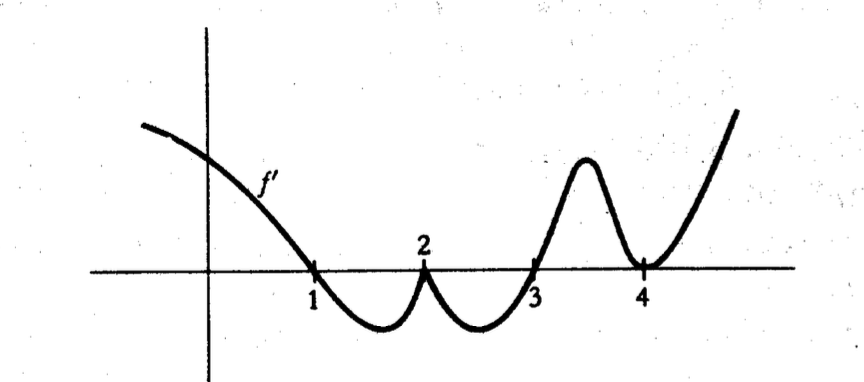
\includegraphics[width=0.5\textwidth]{odvod}
% \caption{Graf odvoda funkcije $f$.}
% \end{figure}
% 	\end{questions}
% \pagestyle{empty}
% \clearpage


% %%%%%%%%%%%%%%%%%%%%%%%%%%%%%%%%%%%%%%%%%%%%%%%%%%%%%%%


% \chead{Matematična analiza 2024/2025 \\ Univerza v Ljubljani, Pedagoška fakulteta \\ Vaje 5 \\20. in 21. marec 2025}
% \pagestyle{head}
% \paragraph{Ključni pojmi}: nedoločene integrale, grafi funkcij.
\section*{Vaje (20. in 21. marec 2025)}

\begin{questions}

\question Izračunaj naslednje nedoločene integrale:
\begin{parts}
\part $\int (2x^4 + x + 2x^{-3} + x^{-1} + 2)  dx $
\part $ \int \left( \sqrt[3]{x} \sqrt{x} + \frac{3}{x^2} - \frac{3}{\sqrt[3]{x}} - \frac{1}{x} \right) dx $
\part $ \int \left(e^{2x} - e^{x+1} \right) dx $
\part $ \int \cos\left( 7x + \frac{\pi}{8} \right) dx $
\end{parts}

\question S pomočjo uvedbe nove spremenljivke izračunaj naslednje nedoločene integrale:
\begin{multicols}{2}
\begin{parts}
    \part $ \int (2x+1)^{19} dx $
    \part $ \int 3x \cos(x^2) dx $
    \part $ \int x e^{1-x^2} dx $
    \part $ \int \frac{x^2}{\sqrt{2x+1}} dx $
    \part $ \int \frac{x}{\sqrt[3]{3x^2+2}} dx $
    \part $ \int \frac{x^3}{\sqrt{2+x^2}} dx $
    \part $ \int \frac{\ln(x)+1}{x \sqrt[3]{\ln(x)}} dx $
    \part $ \int \frac{e^x (e^{2x}-2)}{\sqrt{e^x+1}} dx $
    \part $ \int \frac{e^x}{\sqrt{1-e^{2x}}} dx $
    \part $ \int \frac{\sin(x) \cos^2(x)}{\cos(x)+2} dx $
    \part $ \int \frac{\cos^3(x)}{\sqrt[3]{\sin(x)}} dx $
    \part $ \int \frac{\sin^3(x) + \sin(x) \cos^4(x)}{\sqrt[3]{\cos(x)}} dx $
    \part $ \int \frac{\cos^3(x) + 5\cos(x)}{3+2\sin(x)} dx $
    \part $ \int \cos^2(x) dx $
    \part $ \int \text{ch}^2(x) dx $
    \part $ \int \frac{1}{\sqrt{3-x^2}} dx $
    \part $ \int \frac{1}{\sqrt{-x^2+2x+3}} dx $
    \part $ \int \sqrt{1+x^2} dx $
    \part $ \int \sqrt{x^2-4} dx $
    \part $ \int \frac{x^2}{\sqrt{x^2+1}} dx $
\end{parts}
\end{multicols}

\question S pomočjo integracije `per-partes' izračunajte naslednje integrale:
\begin{multicols}{2}
\begin{parts}
    \part $ \int x e^x dx $
    \part $ \int (4x-1) \sin(6x) dx $
    \part $ \int x \cos^2(x) dx $
    \part $ \int \ln(x) dx $
    \part $ \int (2x-3) \ln(x+1) dx $
    \part $ \int (x^2+\sqrt{x}) \ln(2x) dx $
    \part $\int\left( 2x^{2} - 3x + 1 \right)\sin(3x) dx$
		\part $\int\left(x^2 -3x + 1 \right)e^{-2x}dx$
		\part $\int\left(2x^2 -3x + 1 \right)e^{-3x}dx$
		\part $\int x^{10} e^{-x}$
		\part $\int x^{3} (\ln x)^2 dx$
		\part $\int x^{3} (\sin x) dx$
\end{parts}
\end{multicols}

\question Izračunajte nedoločene integrale naslednjih racionalnih funkcij:
\begin{multicols}{2}
\begin{parts}
    \part $ \int \frac{3+x}{1+x} dx $
    \part $ \int \frac{x^2 - 3x + 2}{x+1} dx $
    \part $ \int \frac{x^3 - 2x^2 + 2}{x-1} dx $
    \part $ \int \frac{x^4 + x^2 + 3}{1 + x^2} dx $
    \part $ \int \frac{x+7}{x^2 - x - 2} dx $
    \part $ \int \frac{x^2 + 3x + 4}{x^2 - 1} dx $
    \part $ \int \frac{2}{(x-1)(x+1)^2} dx $
    \part $ \int \frac{x^2 + 9x + 5}{(x+1)^2(x-2)} dx $
    \part $ \int \frac{dx}{2+8x^2} $
    \part $ \int \frac{2}{x^2 + 2x + 2} dx $
    \part $ \int \frac{4x}{x^2+1} dx $
    \part $ \int \frac{2x+2}{x^2 + 2x + 2} dx $
    \part $ \int \frac{4x+3}{x^2 + 2x + 2} dx $
    \part $ \int \frac{x^2 + 2x - 1}{(x^2 + 2x + 3)(x+1)} dx $
    \part $ \int \frac{3x^2 + 4x - 1}{(x^2 + 2x + 3)(2x+1)} dx $
    \part $ \int \frac{x - 11}{(x^2 + 4)(x - 1)} dx $
    \part $ \int \frac{2x^2 + 8x - 7}{x^3 + 2x^2 - 2x + 3} dx $
    \part $ \int \frac{2x^2 + 5x + 8}{x^3 + 4x^2 + 5x} dx $
    \part $ \int \frac{2}{x^3 + 1} dx $
    \part $ \int \frac{1}{(1 + x^2)^4} dx $
\end{parts}
\end{multicols}



\question Izračunajte naslednje nedoločene integrale:
\begin{multicols}{2}
\begin{parts}
    \part $ \int \frac{(e^x - 3)e^x}{(e^x + 1)(e^x + 2)} dx $
    \part $ \int \frac{e^{2x} - 2}{e^x + 1} dx $
    \part $ \int \frac{(\ln x)^2}{x(1 + (\ln x)^2)} dx $
    \part $ \int \frac{\cos x}{(\sin x)^2 - 4} dx $
    \part $ \int (x - 3) \ln(x + 1) dx $
    \part $ \int x \arctan(2x) dx $
    \part $ \int x \arctan(3x + 2) dx $
    \part $ \int x^2 \arctan(2x) dx $
    \part $ \int (x^3 - \sqrt[3]{x}) \ln(2x) dx $
    \part $ \int e^{\sqrt{x}} dx $
    \part $ \int (\arcsin x)^2 dx $
    \part $ \int \sin^3(x) \ln(\cos x) dx $
    \part $ \int x \sin(\sqrt{x}) dx $
    \part $ \int x^2 e^{\sqrt{x}} dx $
    \part $ \int x \ln(1 + x^2) dx $
    \part $ \int \cos(\ln x) dx $
\end{parts}
\end{multicols}

\end{questions}
% \section*{Seminar (predstavitve)}
	% \begin{questions}
	% 		\question V implicitni in parametrični obliko so podane naslednje krivulje:
	% 	\begin{itemize}
	% 			\item $ x(t) = 4\cos(t), \quad y(t) = 3\sin(t), \quad t \in \mathbb{R}$, (elipsa);
	% 			% \item $ x(t) = \pm 4\cosh(t), \quad y(t) = 3\sinh(t), \quad t \in \mathbb{R}$, (hiperbola);
	% 			\item $ x^{\frac{2}{3}} + y^{\frac{2}{3}} = 1$, (asteroida). \textbf{Nasvet}: Parametriziraj z $ x(t) = \cos^3(t), \quad y(t) = \sin^3(t), \quad t \in [0,2\pi] $;
	% 			% \item $ x(t) = \sin(2t), \quad y(t) = \sin(t), \quad t \in \mathbb{R}$;
	% 			% \item $ x(t) = t^2 - 1, \quad y(t) = t(t^2 - 1), \quad t \in \mathbb{R}$;
	% 			% \item $ x(t) = a(t - \sin t), \quad y(t) = a(1 - \cos t), \quad t \in \mathbb{R}, \quad a > 0 $, (cikloda);
	% 			% \item $ x^3 - 3axy + y^3 = 0, \quad a > 0$, (Descartesov list). \textbf{Nasvet}: Vpelji parameter $ t = \frac{x}{y} $;
	% 			% \item $ x = \cos(at), \quad y = \sin(at), \quad z = bt, \quad t \in \mathbb{R}, $ (vijačnica).
	% 	\end{itemize}
	% 	\begin{parts}
	% 		\part Čimbolj natančno narišite krivulje. Nasvet: Skicirajte grafa $x(t)$ in $y(t)$, ter poskusite določiti ekstremne točke, t.j. rešite tenačbi $\dot{x} =0$ in $\dot{y}=0$.
	% 		\part Izračunajte naklon krivulje oziroma $y'=\frac{\dot{y}}{\dot{x}}$. Izberite si neko točko na krivulji in določite tangento na dano krivuljo v tej točki, če obstaja.
	% 	\end{parts}
		
	% 	\question V implicitni ali polarni obliki so podane naslednje krivulje:
	% 	\begin{itemize}
	% 			% \item $ r(\varphi) = \frac{a}{\varphi}, \quad \varphi \in \mathbb{R}^+$, (hiperbolična spirala).
	% 			% \item $r(\varphi) = e^{a\varphi}$, (logaritemska spirala).
	% 			\item $r(\varphi) = \cos(3\varphi), \quad \varphi \in \left[-\frac{\pi}{6}, \frac{\pi}{6} \right] \cup \left[\frac{\pi}{2}, \frac{5\pi}{6} \right] \cup \left[\frac{7\pi}{6}, \frac{9\pi}{6} \right]$.
	% 			\item $r(\varphi) = a(1 + \cos(\varphi)), \quad \varphi \in [-\pi, \pi] $, (kardioida).
	% 			% \item $(x^2 + y^2) = 2a^2(x^2 - y^2), \quad a > 0$, (lemniskata). \textvf{Nasvet}: Vpelji polarne koordinate.
	% 	\end{itemize}
	% 	\begin{parts}
	% 	\part Čimbolj natančno narišite dane krivulje. Nasvet: skicirajte grafe $r(\varphi)$, $x(\varphi)$ in $y(\varphi)$; poskusite določiti ekstremne točke, t.j. rešite enačbi $\dot{x}=0$ in $\dot{y}=0$.
	% 	\part Izračunajte naklon krivulje oziroma $y' =\frac{\dot{y}}{\dot{x}}$. Določite tangento na dano krivulje v točki, ko je kot $\varphi = \frac{\pi}{2}$, če obstaja.
	% 	\end{parts}

	% \end{questions}
% \pagestyle{empty}
% \clearpage


%%%%%%%%%%%%%%%%%%%%%%%%%%%%%%%%%%%%%%%%%%%%%%%%%%%%%%%


% \chead{Matematična analiza 2024/2025 \\ Univerza v Ljubljani, Pedagoška fakulteta \\ Vaje 6 \\27. in 28. marec 2025}
% \pagestyle{head}
% \paragraph{Ključni pojmi:} Integracijske metode.
\section*{Vaje (27. in 28. marec 2025)}
\begin{questions}
	\question Izračunajte nedoločene integrale naslednjih racionalnih funkcij:
\begin{multicols}{2}
\begin{parts}
    % \part $ \int \frac{3+x}{1+x} dx $
    % \part $ \int \frac{x^2 - 3x + 2}{x+1} dx $
    \part $ \int \frac{x^3 - 2x^2 + 2}{x-1} dx $
    \part $ \int \frac{x^4 + x^2 + 3}{1 + x^2} dx $
    \part $ \int \frac{x+7}{x^2 - x - 2} dx $
    \part $ \int \frac{x^2 + 3x + 4}{x^2 - 1} dx $
    \part $ \int \frac{2}{(x-1)(x+1)^2} dx $
    \part $ \int \frac{x^2 + 9x + 5}{(x+1)^2(x-2)} dx $
    \part $ \int \frac{dx}{2+8x^2} $
    \part $ \int \frac{2}{x^2 + 2x + 2} dx $
    \part $ \int \frac{4x}{x^2+1} dx $
    \part $ \int \frac{2x+2}{x^2 + 2x + 2} dx $
    \part $ \int \frac{4x+3}{x^2 + 2x + 2} dx $
    \part $ \int \frac{x^2 + 2x - 1}{(x^2 + 2x + 3)(x+1)} dx $
    \part $ \int \frac{3x^2 + 4x - 1}{(x^2 + 2x + 3)(2x+1)} dx $
    \part $ \int \frac{x - 11}{(x^2 + 4)(x - 1)} dx $
    \part $ \int \frac{2x^2 + 8x - 7}{x^3 + 2x^2 - 2x + 3} dx $
    \part $ \int \frac{2x^2 + 5x + 8}{x^3 + 4x^2 + 5x} dx $
    \part $ \int \frac{2}{x^3 + 1} dx $
    \part $ \int \frac{1}{(1 + x^2)^4} dx $
\end{parts}
\end{multicols}

	\question Izračunajte naslednje nedoločene integrale:
\begin{multicols}{2}
\begin{parts}
    \part $ \int \frac{(e^x - 3)e^x}{(e^x + 1)(e^x + 2)} dx $
    \part $ \int \frac{e^{2x} - 2}{e^x + 1} dx $
    \part $ \int \frac{(\ln x)^2}{x(1 + (\ln x)^2)} dx $
    \part $ \int \frac{\cos x}{(\sin x)^2 - 4} dx $
    \part $ \int (x - 3) \ln(x + 1) dx $
    \part $ \int x \arctan(2x) dx $
    \part $ \int x \arctan(3x + 2) dx $
    \part $ \int x^2 \arctan(2x) dx $
    \part $ \int (x^3 - \sqrt[3]{x}) \ln(2x) dx $
    \part $ \int e^{\sqrt{x}} dx $
    \part $ \int (\arcsin x)^2 dx $
    \part $ \int \sin^3(x) \ln(\cos x) dx $
    \part $ \int x \sin(\sqrt{x}) dx $
    \part $ \int x^2 e^{\sqrt{x}} dx $
    \part $ \int x \ln(1 + x^2) dx $
    \part $ \int \cos(\ln x) dx $
\end{parts}
\end{multicols}	
\end{questions}
% \section*{Seminar (predstavitve)}
% 	\begin{questions}
% 		\question V implicitni in parametrični obliko so podane naslednje krivulje:
% 		\begin{itemize}
% 				\item $ x(t) = 4\cos(t), \quad y(t) = 3\sin(t), \quad t \in \mathbb{R}$, (elipsa);
% 				% \item $ x(t) = \pm 4\cosh(t), \quad y(t) = 3\sinh(t), \quad t \in \mathbb{R}$, (hiperbola);
% 				\item $ x^{\frac{2}{3}} + y^{\frac{2}{3}} = 1$, (asteroida). \textbf{Nasvet}: Parametriziraj z $ x(t) = \cos^3(t), \quad y(t) = \sin^3(t), \quad t \in [0,2\pi] $;
% 				% \item $ x(t) = \sin(2t), \quad y(t) = \sin(t), \quad t \in \mathbb{R}$;
% 				% \item $ x(t) = t^2 - 1, \quad y(t) = t(t^2 - 1), \quad t \in \mathbb{R}$;
% 				% \item $ x(t) = a(t - \sin t), \quad y(t) = a(1 - \cos t), \quad t \in \mathbb{R}, \quad a > 0 $, (cikloda);
% 				% \item $ x^3 - 3axy + y^3 = 0, \quad a > 0$, (Descartesov list). \textbf{Nasvet}: Vpelji parameter $ t = \frac{x}{y} $;
% 				% \item $ x = \cos(at), \quad y = \sin(at), \quad z = bt, \quad t \in \mathbb{R}, $ (vijačnica).
% 		\end{itemize}
% 		\begin{parts}
% 			\part Čimbolj natančno narišite krivulje. Nasvet: Skicirajte grafa $x(t)$ in $y(t)$, ter poskusite določiti ekstremne točke, t.j. rešite tenačbi $\dot{x} =0$ in $\dot{y}=0$.
% 			\part Izračunajte naklon krivulje oziroma $y'=\frac{\dot{y}}{\dot{x}}$. Izberite si neko točko na krivulji in določite tangento na dano krivuljo v tej točki, če obstaja.
% 		\end{parts}
		
% 		\question V implicitni ali polarni obliki so podane naslednje krivulje:
% 		\begin{itemize}
% 				% \item $ r(\varphi) = \frac{a}{\varphi}, \quad \varphi \in \mathbb{R}^+$, (hiperbolična spirala).
% 				% \item $r(\varphi) = e^{a\varphi}$, (logaritemska spirala).
% 				\item $r(\varphi) = \cos(3\varphi), \quad \varphi \in \left[-\frac{\pi}{6}, \frac{\pi}{6} \right] \cup \left[\frac{\pi}{2}, \frac{5\pi}{6} \right] \cup \left[\frac{7\pi}{6}, \frac{9\pi}{6} \right]$.
% 				\item $r(\varphi) = a(1 + \cos(\varphi)), \quad \varphi \in [-\pi, \pi] $, (kardioida).
% 				% \item $(x^2 + y^2) = 2a^2(x^2 - y^2), \quad a > 0$, (lemniskata). \textvf{Nasvet}: Vpelji polarne koordinate.
% 		\end{itemize}
% 		\begin{parts}
% 		\part Čimbolj natančno narišite dane krivulje. Nasvet: skicirajte grafe $r(\varphi)$, $x(\varphi)$ in $y(\varphi)$; poskusite določiti ekstremne točke, t.j. rešite enačbi $\dot{x}=0$ in $\dot{y}=0$.
% 		\part Izračunajte naklon krivulje oziroma $y' =\frac{\dot{y}}{\dot{x}}$. Določite tangento na dano krivulje v točki, ko je kot $\varphi = \frac{\pi}{2}$, če obstaja.
% 		\end{parts}

% 		\question
% \begin{parts}
% \part Naj bo $n$ naravno število. Z integracijo `po delih' (per partes) pokažite, da velja
    
%     \[
%     \int x^n e^{ax} \,dx = \frac{x^n e^{ax}}{a} - \frac{n}{a} \int x^{n-1} e^{ax} \,dx, \quad a \neq 0.
%     \]
    
% \part Pokažite, da velja
%     \[
%     \int (\ln x)^n \,dx = x (\ln x)^n - n \int (\ln x)^{n-1} \,dx. 
% 		\]
    
% \part S pomočjo zgornjih formul izračunajte naslednje integrale:
% 		\begin{multicols}{2}
% 			\begin{itemize}
% 				\item $\int x^3 e^{2x} \,dx.$ 
% 				\item $\int x^2 e^{-x} \,dx.$ 
% 				\item $\int (\ln x)^3 \,dx.$ 
% 				\item $\int (\ln x)^4 \,dx.$ 
% 			\end{itemize}
% 		\end{multicols}	
    
% \part Kot lahko vidite, če bi integrirali  $\int x^3 e^x \,dx$  z integracijo per partes, bi bil rezultat oblike
% 		\[
%     \int x^3 e^x \,dx = A x^3 e^x + B x^2 e^x + C x e^x + D e^x + E.  
% 		\]
    
%    Odvajajte obe strani te enačbe in izračunajte koeficiente  $A, B, C, D$. Na ta način lahko izračunate integral, ne da bi dejansko izvedli integracijo.
    
% \part Dokažite, da če je  $P$  polinom stopnje  $k$ , potem velja
% 		\[
%     \int P(x) e^x \,dx = [P(x) - P'(x) + \dots \pm P^{(k)}(x)] e^x + C.
% 		\]
    
%     Namig: Uporabite lahko podobno idejo kot pri (d)
    
% \part Izračunajte nasledne integrale
% 	\begin{itemize}    
%      \item $\int (x^2 - 3x + 1)e^x \,dx.$ 
%      \item $\int (x^3 - 2x)e^x \,dx.$
%   \end{itemize}
% \end{parts}

% \question Upoštevajte integral 
% \[
% \int \tan(x) = \int \frac{\sin(x)}{\cos(x)}
% \]

% Integral izračunajte z uporabo integracije “per partes”, pri čemer definirajte $u = \frac{1}{\cos(x)}$ in $dv=\sin(x) dx$.

% Kaj se je zgodilo? ali lahko razložite, zakaj se je to zgodilo?
% 	\end{questions}
% \pagestyle{empty}
% \clearpage


%%%%%%%%%%%%%%%%%%%%%%%%%%%%%%%%%%%%%%%%%%%%%%%%%%%%%%%


% \chead{Matematična analiza 2024/2025 \\ Univerza v Ljubljani, Pedagoška fakulteta \\ Vaje 7 \\3. in 4. april 2025}
% \pagestyle{head}
% \paragraph{Ključni pojmi:} Določeni integral, Riemmannova/Darbouxjevega vsota.
\section*{Vaje (3. in 4. april 2025)}
\begin{questions}
	\question Direktno preko definicije Riemannovega oziroma Darbouxjevega integrala (t.j. z Riemannovimi oziroma Darbouxjevimi vsotami) pokažite, da sta konstantna funkcija $f(x) = C$ in linearna funkcija $g(x) = x$ integrabilni na poljubnem intervalu $[a,b]$, ter izračunajte njuna določena integrala $\int_{a}^{b} C dx$ in $\int_{a}^{b} x dx$.

	\question Dana je funkcija $f(x)= x^{3}$.
	\begin{parts}
		\part Naj bo $\mathcal{D}: 0 < \frac{1}{2} < 1 < \frac{5}{4} < \frac{8}{5} < 2$ delitev intervala $[0,2]$. Zapišite zgornjo in spodnjo Darbouxjevo vsoto funkcije $f$ za dano delitev $\mathcal{D}$, ter ju izračunajte. Kaj geometrijsko predstavljata vsoti?
		\part Za poljuben $n \in \mathbb{N}$ naj bo $\mathcal{D}_{n}: 0 < \frac{2}{n} < \frac{4}{n} < \cdots < \frac{2n-2}{n} < 2$ delitev intervala $[0,2]$. Zapišite zgornjo Darbouxjevo vsoto $S(\mathcal{D}_{n})$ in spodnjo Darbouxjevo vsoto $s(\mathcal{D}_{n})$ funkcije $f$ pri dani delitvi $\mathcal{D}_{n}$. Z indukcijo dokažite formulo $\sum_{j=1}^{n}j^{3} = \frac{n^{2}(n+1)^{2}}{4}$, nato pa jo uporabite pri izračunu limit zaporedij $\lim_{n \to \infty} S(\mathcal{D}_{n})$ in $\lim_{n \to \infty} s(\mathcal{D}_{n})$. Koliko pa je $\int_{0}^{2}x^{3}dx$?
	\end{parts}

	% \question Dana je funkcija $f(x) = \sqrt[3]{x}$
	% 	\begin{parts}
	% 		\part Naj bosta $\mathcal{D}: 0 < \frac{1}{4} < 1 < \frac{3}{2} < 3$ in $\mathcal{D'}: 0 < \frac{1}{4} <\frac{1}{2}< 1 < \frac{3}{2} < \frac{8}{3} < 3$ deltvi intervala $[0,3]$. Zapišite zgornji in spodnji Darbouxjevi vsoti funkcije $f$ za delitvi $\mathcal{D}$ in $\mathcal{D}'$, ter jih primerjajte po velikosti.
	% 		\part Za poljubno število $n \in \mathbb{N}$ naj bo $\mathcal{D}_{n}: 0 < \frac{1}{n} < \frac{2}{n} < \cdots < \frac{n-1}{n} < 1$ delitev intervala $[0,1]$. Zapišite zgornjo Darbouxjevo vsoto $S(\mathcal{D}_{n})$ in spodnjo Darbouxjevo vsoto $s(\mathcal{D}_{n})$ funkcije $f$ za dano delitev $\mathcal{D}_{n}$. Razmislite, zakaj obstajata limite zaporedij $\lim_{n \to \infty} s(\mathcal{D}_{n})$ in $\lim_{n \to \infty} S(\mathcal{D}_{n})$, te ju poiščite.
	% 	\end{parts}

		\question Dana je funkcija $f(x) = \frac{1}{1+2x}$
		\begin{parts}
			\part Izračunajte zgornjo in spodnjo Darbouxjevovsoto funkcije $f$ za naslednjo intervala $[1,3]: 1 < \frac{5}{4} < \frac{3}{2} < \frac{7}{4} < \frac{15}{8} < 2 < \frac{8}{3} < 3$. Kaj geometrijsko predstavljata dobljeni vsoti? Vsoti po velikosti primerjaj še z $\int_{1}^{3} f(x)\ dx$.
			\part Za poljubno število $n \in \mathbb{N}$ naj bo $\mathcal{D}_{n}: 0 < \frac{1}{n} < \frac{2}{n} < \cdots < \frac{n-1}{n} < 1$ delitev intervala $[0,1]$. Zapišite zgornjo Darbouxjevo vsoto $S(\mathcal{D}_{n})$ in spodnjo Darbouxjevo vsoto $s(\mathcal{D}_{n})$ funkcije $f$ za dano delitev $\mathcal{D}_{n}$. Razmislite, zakaj obstajata limite zaporedij $\lim_{n \to \infty} s(\mathcal{D}_{n})$ in $\lim_{n \to \infty} S(\mathcal{D}_{n})$, ter ju izračunajte.
			\part Za $n \in \mathbb{N}$ naj bo $ \mathcal{D}_{n}': 0 < 1 <2 < \cdots < n-1 < n $ delitev intervala $[0,n]$. Zapišite zgornjo in spodnjo Darbouxjevo vsoto funkcije pri dani delitvi $\mathcal{D}_{n}'$. Dobljeni vsoti nato po velikosti primerjajte z določenim integralom $\int_{0}^{n} f(x)\ dx$, ter s pomočjo ugotovljenega pokažite neenakost: 
			\[ 1 + \frac{1}{2} \ln (2n+1) \geq 1 + \frac{1}{3} + \frac{1}{5} + \cdots + \frac{1}{2n+1} \geq \frac{1}{2} \ln (2n+3), \quad n \in \mathbb{N}.\]
		\end{parts}

			\question Dana je funkcija
			\[
			g(x)=
				\begin{cases}
					1, &x \neq 0;  \\
					0,	 & x = 0.
				\end{cases}
			\]
			\begin{parts}
				\part Naj bo $\mathcal{D}: -1 < -\frac{2}{3} < \frac{1}{2} < 1 < 2$ delitev intervala $[-1,2]$. Izračunajte zgornjo in spodnjo Darbouxjevo vsoto funkcije $g$ za dano delitev $\mathcal{D}$.
				\part Direktno po definiciji pokažite (t.j. z Darbouxjevimi vsotami), da je funkcija $g$ integrabilna na intervalu $[-1,2]$, ter $\int_{-1}^{2} g(x)\ dx = 3$.
		\end{parts}

		\question Dana je funkcija
			\[
			h(x)=
				\begin{cases}
					0, &x \in \mathbb{Q};  \\
					1,	 & \mathbb{R}\setminus \mathbb{Q}.
				\end{cases}
			\]
			\begin{parts}
				\part Zapišite zgornjo in spodnjo Darbouxjevo vsoto funkcije $h$ za delitev intervala $[0,2]: 0 < \frac{1}{3} < \frac{2}{3} < \frac{3}{4} < 1 < \frac{3}{2} < 2 $.

				\part Direktno po definiciji pokažite (t.j. z Darbouxjevimi vsotami), da funkcija $h$ ni integlabilna na nobenem zaprtem intervalu. (Nasvet: Upoštevajte, da lahko na vsakem intervalu najdemo tako racionalno kot iracionalno število.)
		\end{parts}

		% \question  Dana je funkcija 
		% \[
		% 	f(x)=
		% 		\begin{cases}
		% 			1, &x >0;  \\
		% 			0,	 & \leq 0.
		% 		\end{cases}
		% 	\]
		% 	\begin{parts}
		% 		\part Zapišite zgornjo in spodnjo Darbouxjevo vsoto funkcije $f$ za delitev intervala $[-1,2]: -1 < -\frac{2}{3} < - \frac{1}{3} < \frac{1}{2} < \frac{3}{2} < 2$.
		% 		\part Direktno po definiciji (t.j. z Darbouxjevimi vsotami) pokažite, da je funkcija $f$ integrabilna na intervalu $[-1,2]$ in velja $\int_{-1}^{2} f(x)\ dx = 2$.
		% 	\end{parts}

			\question S pomočjo določenega integrala izračunajte naslednje limite:
			\begin{parts}
				\part $\displaystyle \lim_{n \to \infty} \left( \frac{1}{n+1} + \frac{1}{n+2} + \cdots + \frac{1}{2n} \right)$
				\part $\displaystyle \lim_{n \to \infty} \frac{\sqrt{1} + \sqrt{2} + \cdots + \sqrt{n}}{\sqrt{n^{3}}}$
				\part $\displaystyle \lim_{n \to \infty} \frac{1 + \sqrt[n]{e} + \sqrt[n]{e^{2}} + \cdots + \sqrt[n]{e^{n-1}} }{n}$
			\end{parts}

			% \question Dana je funkcija $f:[a,b] \to \mathbb{R}$ in delitev $\mathcal{D}: a = x_{0} < \cdots < x_{n} = b$. 
			% \begin{parts}
			% 	\part Za dano delitev intervala $\mathcal{D}$ in funkcijo $f$ definiramo izraz \[T(\mathcal{D}, f) = \sum_{i=1}^{n} \frac{1}{2} \left( f(x_{i}) + f(x_{i+1}) \right)\left(x_{i} - x_{i-1} \right).\]
			% 	Kaj geometrijsko predstavlja zgornja vsota?
			% 	\part Pokažite, da v posebnem primeru, ko so podintervali dane delitve enako veliki (t.j. $x_{i} - x_{i-1} = \frac{b-a}{n}$ za vse $i \in \left\{ 1, \dots, n \right\}$) velja \emph{trapezna formula}:
			% 	\[T(\mathcal{D},f) = \frac{b-a}{2n}\left( f(x_{0}) + 2 f(x_{1}) + 2 f(x_{2}) + \cdots + 2 f(x_{n-1}) + f(x_{n}) \right).\]
			% 	\part Izračunajte $T(\mathcal{D},f)$ za funkcijo $f(x) = e^{-x^{2}}$ in delitev intervala $[0,1]$ na šest enakih podintervalov, $\mathcal{D}: 0 < \frac{1}{6} < \frac{2}{6} < \frac{3}{6} < \frac{4}{6} < \frac{5}{6} < 1$. 
			% \end{parts}

				\question Dokažite, da so naslednje funkcije odvedljive in izračunajte njihove odvode: 
				\begin{parts}
					\part $\displaystyle F(x) = \int_{0}^{x} e^{-t^{3}} dt$, $x \in [0,1]$;
					\part $\displaystyle F(x) = \int_{2}^{2x} e^{-t^{3}} dt$, $x \in [2,4]$;
					\part $\displaystyle F(x) = \int_{0}^{x^{2}} \sin(t^{2}) dt$;
					\part $\displaystyle F(x) = \int_{0}^{x^{2}} f(t) dt$, kjer je $f$ zvezna funkcija na $[0,1]$.
				\end{parts}
				Nasvet: Spomnite se, da je funkcija $F(x) = \int_{a}^{x} f(t) dt$ odvedljiva, ter velja $F'(x) = f(x)$, če je $f$ zvezna. Vpeljite še ustrezno novo spremenljivko ali zapišite $F$ kot ustrezni kompozitum funkcij $F(x) = (G \circ g)(x)$, ter odvajajte po verižnem pravilu.

				\question Izračunajte določeni integral $\int_{0}^{2}f(x) dx$, kjer je 
				\[f(x) = \begin{cases}
					x e^{1-x^{2}}, & x \leq 1; \\
					\sin\left( \frac{\pi x}{2} \right), & x > 1
				\end{cases}.\]

\end{questions}
% \section*{Seminar (predstavitve)}
% 	\begin{questions}
% 		\question
% 	\end{questions}
% \pagestyle{empty}
% \clearpage


%%%%%%%%%%%%%%%%%%%%%%%%%%%%%%%%%%%%%%%%%%%%%%%%%%%%%%%


% \chead{Matematična analiza 2024/2025 \\ Univerza v Ljubljani, Pedagoška fakulteta \\ Vaje 8 \\10. in 11. april 2025}
% \pagestyle{head}
% \paragraph{Ključni pojmi:}Določeni integral, Riemmannova/Darbouxjevega vsota, osnovni izrek integralskega računa.

\section*{Vaje (10. in 11. april 2025)}
\begin{questions}
	\question Dana je funkcija $f(x)= x^{3}$.
	\begin{parts}
		\part Naj bo $\mathcal{D}: 0 < \frac{1}{2} < 1 < \frac{5}{4} < \frac{8}{5} < 2$ delitev intervala $[0,2]$. Zapišite zgornjo in spodnjo Darbouxjevo vsoto funkcije $f$ za dano delitev $\mathcal{D}$, ter ju izračunajte. Kaj geometrijsko predstavljata vsoti?
		\part Za poljuben $n \in \mathbb{N}$ naj bo $\mathcal{D}_{n}: 0 < \frac{2}{n} < \frac{4}{n} < \cdots < \frac{2n-2}{n} < 2$ delitev intervala $[0,2]$. Zapišite zgornjo Darbouxjevo vsoto $S(\mathcal{D}_{n})$ in spodnjo Darbouxjevo vsoto $s(\mathcal{D}_{n})$ funkcije $f$ pri dani delitvi $\mathcal{D}_{n}$. Z indukcijo dokažite formulo $\sum_{j=1}^{n}j^{3} = \frac{n^{2}(n+1)^{2}}{4}$, nato pa jo uporabite pri izračunu limit zaporedij $\lim_{n \to \infty} S(\mathcal{D}_{n})$ in $\lim_{n \to \infty} s(\mathcal{D}_{n})$. Koliko pa je $\int_{0}^{2}x^{3}dx$?
	\end{parts}


	\question Dana je funkcija $f(x) = \sqrt[3]{x}$
		\begin{parts}
			\part Naj bosta $\mathcal{D}: 0 < \frac{1}{4} < 1 < \frac{3}{2} < 3$ in $\mathcal{D'}: 0 < \frac{1}{4} <\frac{1}{2}< 1 < \frac{3}{2} < \frac{8}{3} < 3$ delitvi intervala $[0,3]$. Zapišite zgornji in spodnji Darbouxjevi vsoti funkcije $f$ za delitvi $\mathcal{D}$ in $\mathcal{D}'$, ter jih primerjajte po velikosti.
			\part Za poljubno število $n \in \mathbb{N}$ naj bo $\mathcal{D}_{n}: 0 < \frac{1}{n} < \frac{2}{n} < \cdots < \frac{n-1}{n} < 1$ delitev intervala $[0,1]$. Zapišite zgornjo Darbouxjevo vsoto $S(\mathcal{D}_{n})$ in spodnjo Darbouxjevo vsoto $s(\mathcal{D}_{n})$ funkcije $f$ za dano delitev $\mathcal{D}_{n}$. Razmislite, zakaj obstajata limite zaporedij $\lim_{n \to \infty} s(\mathcal{D}_{n})$ in $\lim_{n \to \infty} S(\mathcal{D}_{n})$, te ju poiščite.
		\end{parts}

		\question  Dana je funkcija 
		\[
			f(x)=
				\begin{cases}
					1, &x >0;  \\
					0,	 & \leq 0.
				\end{cases}
			\]
			\begin{parts}
				\part Zapišite zgornjo in spodnjo Darbouxjevo vsoto funkcije $f$ za delitev intervala $[-1,2]: -1 < -\frac{2}{3} < - \frac{1}{3} < \frac{1}{2} < \frac{3}{2} < 2$.
				\part Direktno po definiciji (t.j. z Darbouxjevimi vsotami) pokažite, da je funkcija $f$ integrabilna na intervalu $[-1,2]$ in velja $\int_{-1}^{2} f(x)\ dx = 2$.
			\end{parts}

			\question Z uporabo osnovnega izreka integralskega računa, določite naslednje integrale.
				\begin{multicols}{3}
					\begin{parts}
						\part $\displaystyle \int_1^2 (x^2 - 2x + 3)\, dx$
						\part $\displaystyle \int_0^8 \left( \sqrt{2x} + \sqrt[3]{x} \right)\, dx$
						\part $\displaystyle \int_1^4 \frac{1 + \sqrt{y}}{y^2} \, dy$
						\part $\displaystyle \int_2^6 \sqrt{x - 2} \, dx$
						\part $\displaystyle \int_0^3 \frac{dx}{\sqrt{25 + 3x}}$
						\part $\displaystyle \int_{-2}^{-3} \frac{dx}{x^2 - 1}$
						\part $\displaystyle \int_0^1 \frac{x \, dx}{x^2 + 3x + 2}$
						\part $\displaystyle \int_{-1}^1 \frac{y^6 \, dy}{y + 2}$
						\part $\displaystyle \int_0^1 \frac{dx}{x^2 + 4x + 5}$
						\part $\displaystyle \int_3^4 \frac{dx}{x^3 - 3x + 2}$
						\part $\displaystyle \int_0^1 \frac{z^3}{z^8 + 1} \, dz$
						\part $\displaystyle \int_{\frac{\pi}{6}}^{\frac{\pi}{4}} \sec^2 a \, da$
					\end{parts}
				\end{multicols}
	
			
				\question Izračunajte določeni integral $\int_{0}^{2}f(x) dx$, kjer je 
				\[f(x) = \begin{cases}
					x e^{1-x^{2}}, & x \leq 1; \\
					\sin\left( \frac{\pi x}{2} \right), & x > 1
				\end{cases}.\]
	
			\question Dokažite, da so naslednje funkcije odvedljive in izračunajte njihove odvode: 
				\begin{parts}
					\part $\displaystyle F(x) = \int_{0}^{x} e^{-t^{3}} dt$, $x \in [0,1]$;
					\part $\displaystyle F(x) = \int_{2}^{2x} e^{-t^{3}} dt$, $x \in [2,4]$;
					\part $\displaystyle F(x) = \int_{0}^{x^{2}} \sin(t^{2}) dt$;
					\part $\displaystyle F(x) = \int_{0}^{x^{2}} f(t) dt$, kjer je $f$ zvezna funkcija na $[0,1]$.
				\end{parts}
				Nasvet: Spomnite se, da je funkcija $F(x) = \int_{a}^{x} f(t) dt$ odvedljiva, ter velja $F'(x) = f(x)$, če je $f$ zvezna. Vpeljite še ustrezno novo spremenljivko ali zapišite $F$ kot ustrezni kompozitum funkcij $F(x) = (G \circ g)(x)$, ter odvajajte po verižnem pravilu.


\end{questions}
% \section*{Seminar (predstavitve)}
% 	\begin{questions}

% 		\question Dana je funkcija $f:[a,b] \to \mathbb{R}$ in delitev $\mathcal{D}: a = x_{0} < \cdots < x_{n} = b$. 
% 		\begin{parts}
% 			\part Za dano delitev intervala $\mathcal{D}$ in funkcijo $f$ definiramo izraz \[T(\mathcal{D}, f) = \sum_{i=1}^{n} \frac{1}{2} \left( f(x_{i}) + f(x_{i-1}) \right)\left(x_{i} - x_{i-1} \right).\]
% 			Kaj geometrijsko predstavlja zgornja vsota?
% 			\part Pokažite, da v posebnem primeru, ko so podintervali dane delitve enako veliki (t.j. $x_{i} - x_{i-1} = \frac{b-a}{n}$ za vse $i \in \left\{ 1, \dots, n \right\}$) velja \emph{trapezna formula}:
% 			\[T(\mathcal{D},f) = \frac{b-a}{2n}\left( f(x_{0}) + 2 f(x_{1}) + 2 f(x_{2}) + \cdots + 2 f(x_{n-1}) + f(x_{n}) \right).\]
% 			\part Izračunajte $T(\mathcal{D},f)$ za funkcijo $f(x) = e^{-x^{2}}$ in delitev intervala $[0,1]$ na šest enakih podintervalov, $\mathcal{D}: 0 < \frac{1}{6} < \frac{2}{6} < \frac{3}{6} < \frac{4}{6} < \frac{5}{6} < 1$. 
% 		\end{parts}

% 		\question S pomočjo določenega integrala izračunajte naslednje limite:
% 			\begin{parts}
% 				\part $\displaystyle \lim_{n \to \infty} \left( \frac{1}{n+1} + \frac{1}{n+2} + \cdots + \frac{1}{2n} \right)$
% 				\part $\displaystyle \lim_{n \to \infty} \frac{\sqrt{1} + \sqrt{2} + \cdots + \sqrt{n}}{\sqrt{n^{3}}}$
% 				\part $\displaystyle \lim_{n \to \infty} \frac{1 + \sqrt[n]{e} + \sqrt[n]{e^{2}} + \cdots + \sqrt[n]{e^{n-1}} }{n}$
% 			\end{parts}

	
% 	\end{questions}
% \pagestyle{empty}
% \clearpage


%%%%%%%%%%%%%%%%%%%%%%%%%%%%%%%%%%%%%%%%%%%%%%%%%%%%%%%



% \chead{Matematična analiza 2024/2025 \\ Univerza v Ljubljani, Pedagoška fakulteta \\ Vaje 9 \\17. in 18. april 2025}
% \pagestyle{head}
% \paragraph{Ključni pojmi:} Uporaba integrala v geometriji in fiziki, izlimitirani integral.

\section*{Vaje (17. in 18. april 2025)}

\begin{questions}
	\question Utemeljite, zakaj so naslednji integrali posplošeni in jih izračunaj, če lahko:
	\begin{multicols}{2}
		\begin{parts}
			\part $\int_0^1 \frac{dx}{\sqrt{x}}$
			\part $\int_{-\infty}^0 \frac{dx}{x - 1}$
			\part $\int_e^\infty \frac{dx}{x \ln(x)}$
			\part $\int_0^1 \frac{dx}{(x - 2)\sqrt{1 - x}}$
			\part $\int_0^\infty \frac{dx}{4 + x^2}$
			\part $\int_{-\infty}^0 e^{2x}(x^2 - 2x)\,dx$
			\part $\int_0^{1/2} \frac{dx}{x(3 - \ln x)}$
			\part $\int_0^1 \frac{dx}{x(3 - \ln x)^2}$
			\part $\int_1^\infty \frac{2dx}{x^2 - 4x + 5}$
			\part $\int_0^\infty \frac{2x + 5}{x^3 - 4x^2 + 5x}\,dx$
		\end{parts}
	\end{multicols}

	\question Raziščite konvergenco oziroma obstoj naslednjih posplošenih integralov:
	\begin{multicols}{2}
		\begin{parts}
			\part $\int_1^\infty \frac{dx}{2x + \sqrt[3]{x^2}}$
			\part $\int_0^1 \frac{e^x dx}{(x - 1)^2}$
			\part $\int_0^\infty \sin(x)\,dx$
			\part $\int_0^1 \frac{\sin x}{\sqrt{x}}\,dx$
			\part $\int_0^\pi \frac{\sin x}{x^2}\,dx$
			\part $\int_0^\infty \frac{\arctg(x)}{(x + 2)^3}\,dx$
			\part $\int_{-\infty}^1 \frac{e^x dx}{(x - 1)^2}$
		\end{parts}
	\end{multicols}

		\question 
		\begin{parts}
			\part Z uporabo integracija izračunajte ploščine trikotnika z danimi oglišči.
			\begin{itemize}
				\part $(0, 0), (1, 3), (3, 1)$.
				\part $(0, 1), (2, 0), (3, 4)$.
			\end{itemize}		
			\part Z uporabo integracija izračunajte ploščine trapeza z oglišči $(-2, -2), (1, 1), (5, 1), (7, -2)$.
		\end{parts}

		

		\question Izračunajte ploščino lika, ki ga omejujejo naslednje krivulje:
\begin{parts}
  \part $y = e^{-x},\ x = -1$ in $y = 1$,
  % \part $y = x^2 - 4$ in $y = -x^2 + 2x$,
  \part $y = xe^{x^{-1}},\ y = 0$ in $x = 1$,
  % \part $y = \sqrt[3]{x}$ in $y = x^2$,
  \part $y = \frac{1}{1+x^2}$ in $y = \frac{x^2}{2}$,
  % \part $y = \sqrt{3x},\ y = -x + 6$ in $y = 0$,
  \part $y = x \ln(x),\ x = 1,\ x = e$ in $y = 0$,
  % \part $f(x) = \sqrt[3]{x},$ tangenta na graf funkcije $f$ v točki $(4,8),$ ter $x$-os,
  \part $f(x) = \ln(x) + 1,$ tangenta na graf funkcije $f$ v točki $(1,1)$ in $x$-os,
  \part $f(x) = -\frac{x^2}{2} + x$ in tangenti na graf funkcije $f$ v točkah $(0,0)$ in $(2,0)$.
\end{parts}

\question Izračunaj dolžino krivulje oziroma obseg lika, določenega z
\begin{parts}
  \part $y = x\sqrt{x}$ in $y = 2x$,
  \part $y = \frac{2}{3}(2 - x)^{\frac{3}{2}},\ x \in [-1,2]$,
  \part $y = \frac{x^2}{4} - \frac{\ln(x)}{2},\ x \in [1,e]$,
  % \part $y = \mathrm{ch}x,\ x \in [-1,1]$,
  \part $y = \sqrt{3x},\ y = -x + 6$ in $y = 0$,
\end{parts}

\question Izračunaj volumen vrtenine, ki jo dobimo, če okrog $x$-osi zavrtimo lik, ki ga omejujejo krivulje z enačbami:
\begin{parts}
  \part $y = \frac{2}{x^2}$ za $x \in [1,4]$,
  % \part $y = xe^{x^{-1}},\ y = 0$ in $x = 1$,
  \part $y = \ln(x),\ x = e$ in $y = 0$,
  % \part $y = \sqrt{4 - x^2}$ in premica $y = 0$,
  \part $y = \sin(x)$ za $x \in [0,\pi]$ in $y = 0$,
  % \part $y = x\sqrt{x}$ in $y = 2x$,
  \part $y = \sqrt{3x},\ y = -x + 6$ in $y = 0$,
  % \part $f(x) = x \ln(x),\ x = e$ in $y = 0$,
\end{parts}

\question Izračunaj površino vrtenine, ki jo dobimo, če okrog $x$-osi zavrtimo lik, ki ga omejujejo krivulje z enačbami:
\begin{parts}
  \part $y = \sqrt{2 - x^2}$ in $y = 1$,
  \part $y = \sqrt{2x},\ x = 2$ in $y = 0$,
  \part $y = \sqrt{3x},\ y = -x + 6$ in $y = 0$,
  % \part $y = \mathrm{ch}(x),\ x \in [-1,1]$.
\end{parts}
	
\end{questions}


% \section*{Seminar (predstavitve)}
% 	\begin{questions}
% 		\question \emph{Gabrielov rog} (znan tudi kot \emph{Torricellijeva trobenta}) je ploskev, ki jo dobimo, če graf funkcije $f(x) = 1/x$ ($x \geq 1$) zavrtimo okoli $x$-osi. 
% 		\begin{parts}
% 			\part Določite površino Gabrielovega roga.
% 			\part Določite prostornino, ki jo zapira Gabrielov rog.
% 		\end{parts}

% 		\question S pomočjo integlalnega računa izpeljite formulo za prostornino in površino piramide, stožca oziroma krogelnega odseka.
% 	\end{questions}
% \pagestyle{empty}
% \clearpage


%%%%%%%%%%%%%%%%%%%%%%%%%%%%%%%%%%%%%%%%%%%%%%%%%%%%%%%


% \chead{Matematična analiza 2024/2025 \\ Univerza v Ljubljani, Pedagoška fakulteta \\ Vaje 10 \\24. in 25. april 2025}
% \pagestyle{head}
% \paragraph{Ključni pojmi:} Uporaba integrala v geometriji in fiziki, izlimitirani integral.	
\section*{Vaje (24. in 25. april 2025)}
\begin{questions}
	\question Utemeljite, zakaj so naslednji integrali posplošeni in jih izračunaj, če lahko:
	\begin{multicols}{2}
		\begin{parts}
			% \part $\int_0^1 \frac{dx}{\sqrt{x}}$
			% \part $\int_{-\infty}^0 \frac{dx}{x - 1}$
			% \part $\int_e^\infty \frac{dx}{x \ln(x)}$
			% \part $\int_0^1 \frac{dx}{(x - 2)\sqrt{1 - x}}$
			% \part $\int_0^\infty \frac{dx}{4 + x^2}$
			\part $\int_{-\infty}^0 e^{2x}(x^2 - 2x)\,dx$
			\part $\int_0^{1/2} \frac{dx}{x(3 - \ln x)}$
			\part $\int_0^1 \frac{dx}{x(3 - \ln x)^2}$
			\part $\int_1^\infty \frac{2dx}{x^2 - 4x + 5}$
			\part $\int_0^\infty \frac{2x + 5}{x^3 - 4x^2 + 5x}\,dx$
		\end{parts}
	\end{multicols}

	\question 
	\begin{parts}
		\part Z uporabo integracija izračunajte ploščine trikotnika z danimi oglišči.
		\begin{itemize}
			\part $(0, 0), (1, 3), (3, 1)$.
			\part $(0, 1), (2, 0), (3, 4)$.
		\end{itemize}		
		\part Z uporabo integracija izračunajte ploščine trapeza z oglišči $(-2, -2), (1, 1), (5, 1), (7, -2)$.
	\end{parts}


	\question Izračunajte ploščino lika, ki ga omejujejo naslednje krivulje:
\begin{parts}
  % \part $y = e^{-x},\ x = -1$ in $y = 1$,
  \part $y = x^2 - 4$ in $y = -x^2 + 2x$,
  % \part $y = xe^{x^{-1}},\ y = 0$ in $x = 1$,
  \part $y = \sqrt[3]{x}$ in $y = x^2$,
  % \part $y = \frac{1}{1+x^2}$ in $y = \frac{x^2}{2}$,
  \part $y = \sqrt{3x},\ y = -x + 6$ in $y = 0$,
  % \part $y = x \ln(x),\ x = 1,\ x = e$ in $y = 0$,
  \part $f(x) = \sqrt[3]{x},$ tangenta na graf funkcije $f$ v točki $(4,8),$ ter $x$-os,
  % \part $f(x) = \ln(x) + 1,$ tangenta na graf funkcije $f$ v točki $(1,1)$ in $x$-os,
  \part $f(x) = -\frac{x^2}{2} + x$ in tangenti na graf funkcije $f$ v točkah $(0,0)$ in $(2,0)$.
\end{parts}

\question Izračunaj volumen vrtenine, ki jo dobimo, če okrog $x$-osi zavrtimo lik, ki ga omejujejo krivulje z enačbami:
\begin{parts}
  % \part $y = \frac{2}{x^2}$ za $x \in [1,4]$,
  \part $y = xe^{x^{-1}},\ y = 0$ in $x = 1$,
  % \part $y = \ln(x),\ x = e$ in $y = 0$,
  \part $y = \sqrt{4 - x^2}$ in premica $y = 0$,
  % \part $y = \sin(x)$ za $x \in [0,\pi]$ in $y = 0$,
  \part $y = x\sqrt{x}$ in $y = 2x$,
  % \part $y = \sqrt{3x},\ y = -x + 6$ in $y = 0$,
  \part $f(x) = x \ln(x),\ x = e$ in $y = 0$,
\end{parts}

\question 
Naj bo $a > 0$. Izračunajte dolžino dela krivulje:
\begin{parts}
	\part $f(x) = \frac{x^{2}}{4}-\frac{\ln x }{2}$ nad intevalom $[1,e]$. 
	% \part $f(x) = \ln ( 1-x^{2})$ nad intervalom $\left[ 0, \frac{1}{2} \right]$. 
	\part $x(t) = a(t-\sin t)$, $y=a(1 - \cos t)$ med dvema zaporednima točkama, ki ležita na abscisni osi.
	\part $f(x) = \ln \left( \sin (x-1) \right)$ med točkama $x=1+ \frac{\pi}{3}$ in $x=1+\frac{2 \pi}{3}$.
	\part $r = e^{a \phi}$, $\phi \in \mathbb{R}$, znotraj kroga $x^{2} + y^{2} \leq 1$.
\end{parts}

\question
Krivulja $K$ je podana parametrično z \[x(t) = 4+2 \ln t \quad y(t) = t + \frac{1}{t}, \qquad t > 0.\] Označimo s $T$ točko na krivulji $K$, ki je najbližja abscisni osi. Izračunajte dolžino krivulje $K$ med točko $T$ in točko, kjer krivulja seka premivo $x = 8$.

\question 
Izračunajte obseg in ploščino astroide. Astroida je podana implicitno z enačbo $x^{\frac{2}{3}} + y^{\frac{2}{3}} = a^{\frac{2}{3}}$, $a > 0$.

\end{questions}
% \section*{Seminar (predstavitve)}
% 	\begin{questions}
% 		\question \emph{Gabrielov rog} (znan tudi kot \emph{Torricellijeva trobenta}) je ploskev, ki jo dobimo, če graf funkcije $f(x) = 1/x$ ($x \geq 1$) zavrtimo okoli $x$-osi. 
% 		\begin{parts}
% 			\part Določite površino Gabrielovega roga.
% 			\part Določite prostornino, ki jo zapira Gabrielov rog.
% 		\end{parts}

% 		\question S pomočjo integlalnega računa izpeljite formulo za prostornino in površino piramide, stožca oziroma krogelnega odseka.

% 		\question Naj bo $f: [1, \infty) \to \mathbb{R}$ zvezna funkcija, za katero obstaja integral $ \displaystyle \int_{1}^{\infty} \frac{f^{2}(t)}{t^{2}} dt$.
% 		\begin{parts}
% 			\part Dokažite, da obstaja integral $ \displaystyle \int_{1}^{\infty} \frac{1+ f^{2}(t)}{t^{2}} dt$.
% 			\part Dokažite, da obstaja integral $ \displaystyle \int_{1}^{\infty} \frac{|f(t)|}{t^{2}} dt$.
% 		\end{parts}

% 		\question Naj bo $f: [0, \infty] \to \mathbb{R}$ zvezna funkcija in $\displaystyle \lim_{x \to \infty} f(x) = c \geq 0$.
% 		\begin{parts}
% 			\part Dokažite, da za vsak $a \geq 0$ obstaja takšen $b \geq 0$, da je $\displaystyle \int_{0}^{b} f(t)dt = a$.
% 			\part Dokažite, da obstaja takšen $M \geq 0$, da je za vsak $a \geq M$ število $b$, ki ustreza pogojem iz prejšnje točke, enolično določeno.
% 		\end{parts}
% 		\textbf{Nasvet:} upoštevajte funkcio $F(b)= \displaystyle \int_{0}^{b} f(t) dt$
% 	\end{questions}
% 	\pagestyle{empty}
% % \pagestyle{empty}
% \clearpage


%%%%%%%%%%%%%%%%%%%%%%%%%%%%%%%%%%%%%%%%%%%%%%%%%%%%%%%


% \chead{Matematična analiza 2024/2025 \\ Univerza v Ljubljani, Pedagoška fakulteta \\ Vaje 11 \\8. in 9. maj 2025}
% \pagestyle{head}
% \paragraph{Ključni pojmi:} Zaporedje funkcij, vrste funkcij, konvergenca po točkah, enakomerna konverngenca.
\section*{Vaje (8. in 9. maj 2025)}
\begin{questions}

	\question Dana so naslednja funkcijska zaporedja:
	\begin{multicols}{2}
		\begin{parts}
			\part $f_n(x) = x\left(1 + \frac{1}{n}\right),$
			\part $f_n(x) = \frac{1}{1 + x^{2n}},\ x \in [0,1],$
			\part $f_n(x) = \arctan(nx),$
			\part $f_n(x) = \frac{x}{1 + nx^2},$
			\part $f_n(x) = \frac{nx}{1 + n^2 x^2},$
			\part $f_n(x) = \frac{nx^2 + 1}{nx + 1},\ x \in [0, \infty),$
			\part $f_n(x) = xe^{-nx},$
			\part $h_{n}(x) = 2xn^2 e^{-n^2 x^2},$
			\part $h_{n}(x) = \frac{1}{n} e^{-n^2 x^2},$
			\part $f_n(x) = \frac{\sin(nx)}{n}.$
		\end{parts}
	\end{multicols}
	
	\begin{itemize}
		\item Ugotovite, ali dano zaporedje funkcij konvergira po točkah oziroma enakomerno, ter izračunaj limito $f(x) = \lim_{n \to \infty} f_n(x)$, če obstaja.
		\item Ali zaporedje odvodov $f_n'(x)$, če obstajajo, konvergira po točkah oziroma enakomerno? Če je odgovor pritrdilen, poiščite tudi limito. Ali je enaka odvodu limitne funkcije zaporedja $f_n$?
		\item Ali konvergira zaporedje integralov $\int_0^1 f_n(x) \, dx$, t.j. ali obstaja limita $\lim_{n \to \infty} \int_0^1 f_n(x) \, dx$; je morda enaka $\int_0^1 (\lim_{n \to \infty} f_n(x)) \, dx$?
	\end{itemize}
	
	\question Določite konvergenčne polmere oziroma območja konvergence naslednjih potenčnih vrst oziroma funkcijskih vrst (raziščite tudi konvergenco na robu območij):
	\begin{multicols}{2}
		\begin{parts}
			\part $\sum_{n=1}^\infty \frac{x^n}{n},$
			\part $\sum_{n=0}^\infty (n+1)x^n,$
			\part $\sum_{n=0}^\infty \frac{n}{2^n}(x - 2)^n,$
			\part $\sum_{n=1}^\infty \frac{\cos(nx)}{10^n},$
			\part $\sum_{n=1}^\infty e^{-nx},$
			\part $\sum_{n=1}^\infty \frac{1}{n^x}.$
		\end{parts}
	\end{multicols}
	
	\end{questions}
	


% \section*{Seminar (predstavitve)}
% 	\begin{questions}
% 		\question Naj bosta $\left\{ f_{n} : D \to \mathbb{R}\right\}$ in $\left\{ g_{n}: D \to \mathbb{R}\right\}$ zaporediji funkcij. Prepostavite, da $\left\{ f_{n}\right\}$ in $\left\{ g_{n}\right\}$ konvergirata enakomerno na $D$.  
% 		\begin{parts}
% 			\part Dokažite, da je zaporedja funkcij $\left\{ f_{n} + g_{n} \right\}$.
% 			\part Dokažite, da če sta $\{f_{n}\}$ in $\{g_{n}\} $ zaporedji omejenih funkcij, potem je zaporedje $\{f_{n}g_{n}\}$ enakomerno konvergira.
% 			\part Poiščite zaporedji funkcij $\{f_{n}\}$ in $\{g_{n}\}$, ki enakomerno konvergirata na neki množici $D$, vendar tako $\{f_{n} g_{n}\}$ konvergira po točkah na $D$, vendar ne konvergira enakomerno na $D$.  
% 		\end{parts}

% 		\question 
% 		\begin{parts}
% 			\part Za $n \in \mathbb{N}$ in $x \in \mathbb{R}$, naj bo \[f_{n}(x) = \frac{x}{1+nx^{2}}.\]  Dokažite, da zaporedja funkcij $\left\{ f_{n} \right\}$ enakomerno konvergira proti funkciji $f$, in da \[f'(x) = \lim_{n \to \infty} f_{n}'(x)\] velja, če je $x \neq 0$, pa ne, če je $x=0$.  
% 			\part Obstaja izrek, ki pravi, kdaj velja enačba \[f'(x) = \lim_{n \to \infty} f_{n}'(x)\] za zaporedje funkcij $\left\{ f_{n} \right\}$. Zakaj ta izrek ne drži v prejšnjem primeru?
% 		\end{parts}

% 		\question Dano je zaporedje funkcij $f: [0, \infty) \to \mathbb{R}$, \[f_{n}(x) = \frac{\ln(1+x/n)}{x+1}.\]
% 		\begin{parts}
% 			\part Dokažite, da zapordje konvergira po točkah na $[0, \infty)$, in določi limitno funkcijo.
% 			\part Dokažite, da zaporedje konvergira enakomerno na $[0,a]$ za vsak $a > 0$.
% 			\part Ali je konvergenca enakomerna na $[0, \infty]$? Odgovor utemeljite.
% 		\end{parts}

		
		
% 	\end{questions}
% \pagestyle{empty}
% \clearpage


%%%%%%%%%%%%%%%%%%%%%%%%%%%%%%%%%%%%%%%%%%%%%%%%%%%%%%%




% \chead{Matematična analiza 2024/2025 \\ Univerza v Ljubljani, Pedagoška fakulteta \\ Vaje 12 \\15. in 16. maj 2025}
% \pagestyle{head}
% \paragraph{Ključni pojmi:} Taylorjeve vrste.
\section*{Vaje (15. in 16. maj 2025)}
\begin{questions}
		\question Naslednje funkcije razvijte v Taylorjeve vrste okoli točke $x = a$, določite območja konvergence dobljenih vrst in izračunajte $f^{(2024)}(a)$ in $f^{(2025)}(a)$:
		\begin{parts}
			\part $f(x) = 2x^3 + 3x^2 - x + 1$ okoli točke $a = 1$;
			\part $f(x) = 1 - \cos(2x)$ okoli točke $a = 0$;
			\part $f(x) = xe^{-x}$ okoli točke $a = 0$;
			% \part $h(x) = x^2 \cos(2x)$ okoli točke $a = 0$;
			\part $f(x) = e^{2x}$ okoli točke $a = 2$;
			\part $f(x) = \ln(x)$ okoli točk $a_1 = 1$ in $a_2 = 2$;
			% \part $f(x) = \ln(2 + x)$ okoli točke $a = -1$;
			% \part $f(x) = x(e^{-x} - 1)$ okoli točke $a_1 = 0$;
			\part $f(x) = \frac{1}{1 + x}$ okoli točk $a_1 = 0$ in $a_2 = 1$;
			% \part $h(x) = \frac{1}{3 - x}$ okoli točk $a_1 = 0$ in $a_2 = 2$;
			% \part $g(x) = \frac{1}{4 + x^2}$ okoli točke $a = 0$;
			% \part $r(x) = \frac{1}{x^2 - x}$ v Taylorjevo vrsto okoli točke $a = -1$;
			% \part $s(x) = (1 - x^2)^{-\frac{1}{2}}$ okoli $a = 0$(Zapišite do členov četrtega reda);
			\part $f(x) = \arctg(x)$ okoli točke $a = 0$.
		\end{parts}

		\question S pomočjo Taylorjeve formule ocenite napako naslednjih približkov:
			\begin{parts}
				\part $\displaystyle \frac{1}{1 - x} \approx 1 + x, \qquad |x| < \frac{1}{100}$;
				\part $\sin(x) \approx x, \qquad |x| < \frac{1}{100}$;
				\part $\cos(x) \approx 1 - \frac{x^2}{2}, \qquad |x| < \frac{1}{2}$.
			\end{parts}

			\question Z uporabo Taylorjeve vrste do členov tretjega reda izračunajte približne vrednosti:
			\begin{multicols}{2}
				\begin{parts}
					\part $0,99^{12}$,
					\part $\sqrt{1,01}$,
					\part $\sin(59^\circ)$,
					\part $\arcsin(0,04 + \ln(1,02))$.
				\end{parts}
			\end{multicols}

\question S pomočjo Taylorjeve formule oziroma razvoja v Taylorjevo vrsto izračunajte naslednje limite:
\begin{multicols}{2}
\begin{parts}
  \part $\displaystyle \lim_{x \to 0} \frac{\tan x - x}{x - \sin x},$
  % \part $\displaystyle \lim_{x \to 0} \frac{5 \sin(x) - \sin(5x)}{x^2 \sin x},$
  \part $\displaystyle \lim_{x \to 0} \frac{x(e^x - 1)}{1 - \cos(2x)},$
  % \part $\displaystyle \lim_{x \to 0} \frac{x(e^x - 1)}{1 - \cos(3x)},$
  \part $\displaystyle \lim_{x \to 0} \frac{e^{x^{2}} - 1}{1 - \cos(2x)},$
  % \part $\displaystyle \lim_{x \to 0} \frac{3x - \sin(3x)}{e^{2x} - e^{-2x}},$
  \part $\displaystyle \lim_{x \to 0} \frac{\ln x - \frac{2x -2}{x + 1}}{\sin^3(\pi x)},$
  % \part $\displaystyle \lim_{x \to 0} x^{-4} e^{-\frac{1}{x^2}}.$
\end{parts}
\end{multicols}

\end{questions}
% \section*{Seminar (predstavitve)}
% 	\begin{questions}
% 		\question 
% 		\begin{parts}
% 			\part Za $n \in \mathbb{N}$ in $x \in \mathbb{R}$, naj bo \[f_{n}(x) = \frac{x}{1+nx^{2}}.\]  Dokažite, da zaporedja funkcij $\left\{ f_{n} \right\}$ enakomerno konvergira proti funkciji $f$, in da \[f'(x) = \lim_{n \to \infty} f_{n}'(x)\] velja, če je $x \neq 0$, pa ne, če je $x=0$.  
% 			\part Obstaja izrek, ki pravi, kdaj velja enačba \[f'(x) = \lim_{n \to \infty} f_{n}'(x)\] za zaporedje funkcij $\left\{ f_{n} \right\}$. Zakaj ta izrek ne drži v prejšnjem primeru?
% 		\end{parts}

% 		\question Dano je zaporedje funkcij $f: [0, \infty) \to \mathbb{R}$, \[f_{n}(x) = \frac{\ln(1+x/n)}{x+1}.\]
% 		\begin{parts}
% 			\part Dokažite, da zapordje konvergira po točkah na $[0, \infty)$, in določi limitno funkcijo.
% 			\part Dokažite, da zaporedje konvergira enakomerno na $[0,a]$ za vsak $a > 0$.
% 			\part Ali je konvergenca enakomerna na $[0, \infty]$? Odgovor utemeljite.
% 		\end{parts}

% 		\question
% 		Določite $a,b,c,d \in \mathbb{R}$, da bo obstajala (končna) limita 
% 		\[L = \lim_{x \to 0} \frac{1}{x^{5}}\left( e^{x} - \frac{1+ ax +bx^{2}}{1+cx+dx^{2}} \right)\]

% 		\question
% 		Dokažite, da je število $e$ iracionalno. To storite tako
% 		\begin{parts}
% 			\part Predpostavite, da lahko $e$ zapišemo kot ulomek $\frac{a}{b}$, kjer sta $a,b$ naravni števili.
% 			\part Izberite $n > \max \left\{ 3,b \right\}$ in s pomočjo Taylorjeve vrste, izračunajte približek $e = e^1$ (do $n$-tega reda). Dokažite, da je za napako $R_n$ tega približka $0 < R_{n} < \frac{3}{(n+1)!}$.
% 			\part Zgornji dve točki uporabite za ugotovitev nasprotja s predpostavko $e=\frac{a}{b}$.
% 		\end{parts}
% 	\end{questions}
% \pagestyle{empty}
% \clearpage


%%%%%%%%%%%%%%%%%%%%%%%%%%%%%%%%%%%%%%%%%%%%%%%%%%%%%%%


% \chead{Matematična analiza 2024/2025 \\ Univerza v Ljubljani, Pedagoška fakulteta \\ Vaje 13 \\22. in 23. maj 2025}
% \pagestyle{head}
% \paragraph{Ključni pojmi:} Metrični prostori.	
\section*{Vaje (22. in 23. maj 2025)}

\begin{questions}

	\question Naj bo $(M,d)$ metrični prostor. Dokažite, da za vse $w, x, y, z \in M$ velja neenakost 
		\[
		|d(x,y) - d(z,w)| \leq d(x,z) + d(y,w).
		\]

	\question Naj bosta $d$ in $e$ metriki na množici $M$. 
		\begin{parts}
			\part Naj bo $g: M \times M \to \mathbb{R} $ funkcija
				\[
					(x,y) \mapsto \min\{d(x,y), e(x,y)\}
				\] 
				Pokažite, da $g$ ni nujno metrika na množici $M$ in najdite pogoj, pod katerim je.
			\part Pokažite, da je funckcija $h:  \times M \to \mathbb{R} $ s predpisom
			\[h(x,y) = \max \{d(x,y), e(x,y)\}\] metrika na množici $M$.
			\part Dokažite, da je funkcija $h:M\times M \to \mathbb{R}$ definirana s predpisom $s(x,y) = d(x,y) + e(x,y)$ metrika na množici $M$.
		\end{parts}

		\question Naj bo $X$ končna množica. Naj $M=\mathcal{P}(X)$ označuje množico vseh podmnožic množice $X$. Za $A,B \in M$ naj $A \triangle B$ označuje simetrično razliko množic $A$ in $B$, to je, \[A \triangle B = (A\cup B) \setminus (A \cap B).  \] Definiramo funkcijo $d: M \times M \to \mathbb{R}$ s predpisom $d(A,B) = \left| A \triangle B \right|$.

		\begin{parts}
			\part Dokažite, da je $d$ metrika na množici $M$.
			\part Izračunajte $d(A,B)$ za vsak par podmnožic $A,B \subset \left\{ a,b,c \right\}$.
		\end{parts}
		
		

	\question	V množico $M=(0,\infty) \times (0, \infty)$ vpeljemo $d: M \times M \to \mathbb{R}$ s pravilom \[d\left( (x_{1},y_{1}), (x_{2},y_{2}) \right) = \left| \ln \frac{x_{2}}{x_{1}} \right| + \left| \ln \frac{y_{2}}{y_{1}} \right|.\]

		\begin{parts}
			\part Dokažite, de je $d$ metrika na množici $M$.
			\part Skicirajte odprto kroglo $K((1,1),1)$.
		\end{parts}

		\question Na množico $\mathbb{R}$ vpeljemo metriko $d$ s predpisom 
		\[d(x,y) = 
			\begin{cases}
				|x-y|, & \text{če sta } x,y \in \mathbb{Q}, \text{ ali sta } x,y  \in \mathbb{R} \setminus \mathbb{Q}; \\ 
				|x-y|+1, & \text{sicer}.
			\end{cases}
		\]
		Dokažite, da je $d$ res metrika na množici $\mathbb{R}$ in določite kroglo $K(0,2)$.

		\question Poiščite točke na premici $y = 2x +1$, ki so najbližje izhodišču v metrikah $d_{1}$, $d_{2}$ in $d_{\infty}$.
		Te metrike so podane s predpisomi
		\begin{align*}
			d_{1}\left( (x_{1}, y_{1}), (x_{2}, y_{2}) \right) &= |x_{1} - x_{2}| + |y_{1} - y_{2}| \\
			d_{2}\left( (x_{1}, y_{1}), (x_{2}, y_{2}) \right) &= \sqrt{(x_{1} - x_{2})^{2} + (y_{1} - y_{2})^{2}} \\
			d_{\infty}\left( (x_{1}, y_{1}), (x_{2}, y_{2}) \right) &= \max\left\{ |x_{1} - x_{2}|, |y_{1} - y_{2}| \right\}\\
		\end{align*}

		\question Na množico $M = \mathbb{R}^{2}$ vpeljemo predpis 
		\[d\left( (x_{1}, y_{1}), (x_{2}, y_{2}) \right)=
		\begin{cases}
			|x_{2} - x_{1}|, &\text{če je } y_{1} = y_{2}; \\
			|x_{2} - x_{1}| + |y_{1}| + |y_{2}|, & \text{če } y_{1} \neq y_{2}.
		\end{cases}
		\]
		\begin{parts}
			\part Pokažite, da je $d$ metrika.
			\part Skicirajte zaprti krogli $\bar{K}\left( (0,1),1 \right)$ in $\bar{K}\left( (0,1),2 \right)$.
		\end{parts}

		
	\question Naj bo $M = \mathbb{N} \cup \left\{ \infty \right\}$ in $d: M \times M \to \mathbb{R}$ podana s predpisom:
	\[d(m,n) = 
		\begin{cases}
			\left| \frac{1}{n} - \frac{1}{m} \right|,  & \text{če } n \neq \infty, m\neq \infty; \\
			\frac{1}{n},  & \text{če } n \neq \infty, m =  \infty; \\
			\frac{1}{m},  & \text{če } n = \infty, m\neq \infty; \\
			0,  & \text{če } n = \infty, m = \infty.
		\end{cases}
	\]
	\begin{parts}
		\part Pokažite, da je $(M,d)$ metrični prostor.
		\part Pokažite, da za vsak $n \in \mathbb{N}$ obstaja $r >0$, da je $K(n,r) = \left\{ n \right\}$. 
		Pokažite tudi, da za vsak $r > 0 $ krogla $K(\infty,r)$ vsebuje vse razen končno mnogo elementov $M$.
	\end{parts}

	\question Naj bo $(M,d)$ metrični prostor. Definirajmo \[\bar{d}\left( x,y \right) = \frac{d(x,y)}{1+d(x,y)}.\] Pokažite, da je tudi $\bar{d}$ metrika na množici $M$.


\end{questions}
% \section*{Seminar (predstavitve)}
% 	\begin{questions}
% 		\question Naj bo $X$ poljubna neprazna množica. Označimo z $X^{\mathbb{N}}$ množico vseh zaporedij  $(x_{1}, x_{2}, \dots)$ točk iz $X$. Definirajmo razdaljo $d(x,y)$ dveh elementov $x=(x_{1}, x_{2}, \dots)$ in $y=(y_{1}, y_{2}, \dots)$ te množice takole: \[d(x,y) = \begin{cases} 0, & \text{če je } x=y;  \\ \frac{1}{n} & \text{če veljajo } x_{1}=y_{1}, x_{2}= y_{2}, \dots, x_{n-1} = y_{n-1}, \text{ in } x_{n} \neq y_{n}. \end{cases}\]
% 		\begin{parts}
% 			\part Dokažite, da res je $d$ metrika na množici $M$.
% 			\part Pokažite, da ima ta prostor tole čudno lastnost: vsaka točka poljubne (odprte ali zaprte) krogle je središče te krogle; poleg tega sta vsaki dve krogli bodisi disjunktni ali pa ena od njiju vsebuje drugo.
% 		\end{parts}

% 		\question Naj bo $M=\mathbb{R}[x]$ množica polinomov s koeficienti na realmi števili. Vsak element $p \in \mathbb{R}[x]$ zapišite kot $p = \sum_{i=0}^{\infty} \alpha_i x^{i}$, kjer so vsi koeficienti $\alpha_{i}$, raze knočnega števila, enaki nič. (npr. če je $p = 3x^{3} - 2x +1$,nato $\alpha_{0} = 1$, $\alpha_{1} =- 2$, $\alpha_{2} = 0$, $\alpha_{3} = 3$ in $\alpha_{i} = 0 $ če je $i \geq 4$). Definirajmo razdaljo $d \left( p(x), q(x) \right)$ dveh elementov $p(x) = \sum_{i=0}^{\infty} \alpha_{i} x^{i}$  $p(x) = \sum_{i=0}^{\infty} \beta_{i} x^{i}$ množice $\mathbb{R}[x]$ takole: \[d \left( p(x), q(x) \right) = \sup \left\{ \left| \alpha_{i} - \beta_{i} \right| : 0 \leq i < \infty \right\}.\]
		
% 		Dokažite, da je $d$ metrika na množici $\mathbb{R}[x]$ (pazite!, morate dokazati da je $d \left( p(x), q(x) \right)$ realno število za vsak $p(x), q(x) \in \mathbb{R}[x]$).

% 		\question Naj bo $p$ praštevilo. Vsako nenicelno racionalno število $x$ lahko enolično zapišemo kot $x = p^k \frac{r}{s}$, kjer sta $k \in \mathbb{Z}$, $r \in \mathbb{Z}$ in $s \in \mathbb{N}$, pri čemer $p$ ne deli $r$ in $p$ ne deli $s$. Definiramo $|x|_p = p^{-k}$, in še $|0|_p = 0$.

% 		Definiramo funkcija $d_{p}: \mathbb{Q} \times \mathbb{Q}\to \mathbb{R}$ kot $d_{p}(x,y) \mapsto |x - y|_p$. 
% 		Dokažite da je $d_{p}$ metrika na množici racionalnih števil. 
% 		% To je očitno nenegativna simetrična funkcija, ki je enaka $0$ natanko tedaj, ko je $a = b$. Trikotniško neenakost lahko preverimo na sledeč način: če je $|a - c|_p = p^{-m}$ in $|c - b|_p = p^{-n}$, potem velja
% 			% \[
% 			% |a - b|_p \leq \max\{p^{-m}, p^{-n}\}.
% 			% \]


% 	\end{questions}
% \pagestyle{empty}
% \clearpage
%%%%%%%%%%%%%%%%%%%%%%%%%%%%%%%%%%%%%%%%%%%%%%%%%%%%%%%




% \chead{Matematična analiza 2024/2025 \\ Univerza v Ljubljani, Pedagoška fakulteta \\ Vaje 14 \\29. in 30. maj 2025}
% \pagestyle{head}
% \paragraph{Ključni pojmi:}	Metrični prostor, oprte množice, zaprte množice.
\section*{Vaje (29. in 30. maj 2025)}
\begin{questions}
	\question Naj bodo $d_{1}$, $d_{2}$ in $d_{\infty}$ metrike na množici $\mathbb{R}^{2}$ definirane s predpisi
		\begin{align*}
			d_{1}\left( (x_{1}, y_{1}), (x_{2}, y_{2}) \right) &= |x_{1} - x_{2}| + |y_{1} - y_{2}| \\
			d_{2}\left( (x_{1}, y_{1}), (x_{2}, y_{2}) \right) &= \sqrt{(x_{1} - x_{2})^{2} + (y_{1} - y_{2})^{2}} \\
			d_{\infty}\left( (x_{1}, y_{1}), (x_{2}, y_{2}) \right) &= \max\left\{ |x_{1} - x_{2}|, |y_{1} - y_{2}| \right\}
		\end{align*}
		\begin{parts}
			\part Skicirajte odprta krogla ${K}\left( (0,0),1 \right)$ za vsako od zgornjih metrik.
			\part Poiščite točke na premici $y = 2x +1$, ki so najbližje izhodišču v metrikah $d_{1}$, $d_{2}$ in $d_{\infty}$.
		\end{parts}

	\question Dan je metrični prostor $(M,d)$ in naj bo $Z$ poljubna množica. Prepostavite, da je $f \colon Z \to M$ injektivna funkcija. Pokažite, da je $(a,b) \mapsto d(f(a), f(b))$ metrika na množici $Z$.


	\question Na množico $M = \mathbb{R}^{2}$ vpeljemo predpis 
		\[d\left( (x_{1}, y_{1}), (x_{2}, y_{2}) \right)=
		\begin{cases}
			|x_{2} - x_{1}|, &\text{če je } y_{1} = y_{2}; \\
			|x_{2} - x_{1}| + |y_{1}| + |y_{2}|, & \text{če } y_{1} \neq y_{2}.
		\end{cases}
		\]
		\begin{parts}
			\part Pokažite, da je $d$ metrika.
			\part Skicirajte zaprti krogli $\bar{K}\left( (0,1),1 \right)$ in $\bar{K}\left( (0,1),2 \right)$.
		\end{parts}
		
	\question Ugotovite, ali je $A$ odprta oziroma zaprta podmnožica danega metričnega prostora:
	\begin{parts}
		\part $A = \left\{ \frac{1}{n} : n \in \mathbb{N}\right\} \subset \mathbb{R}$;
		\part $A = \mathbb{Z} \subset \mathbb{R}$;
		\part $A = \mathbb{R}\times \left\{ 0 \right\} = \left\{ (x, 0) : x \in \mathbb{R} \right\} \subset \mathbb{R}^{2}$;
		\part $A = \mathbb{R} \setminus \mathbb{Q} \subset \mathbb{R}$;
		\part $A = \left\{ (k,\ell) : k,\ell \in \mathbb{Z} \right\} \subset \mathbb{R}^{2}$; 
		\part $A = \left\{ (x,y) \in \mathbb{R}^{2} : |x| < |y| \right\} \subset \mathbb{R}^{2}$;
		\part $A = \left\{ (x,y) \in \mathbb{R}^{2} : x^{2} + y^{2} < 1 \right\} \subset \mathbb{R}^{2}$;
		\part $A = \left\{ p \restriction_{[0,1]} : p \in \mathbb{R}[x]\right\} \subset \left( C([0,1]), d_{\infty} \right)$, kjer je $p \restriction_{[0,1]} : [0,1] \to \mathbb{R}$ funkcija definirana s predpisom $p\restriction_{[0,1]} (x) = p(x)$ in metrika $d_{\infty}$ je pa $d_{\infty}(f,g) = \sup \left\{ |f(x) - g(x)| : x \in [0,1] \right\}$.
	\end{parts}

	\question Naj bo $M = \mathbb{N} \cup \left\{ \infty \right\}$ in $d: M \times M \to \mathbb{R}$ podana s predpisom:
	\[d(m,n) = 
		\begin{cases}
			\left| \frac{1}{n} - \frac{1}{m} \right|,  & \text{če } n \neq \infty, m\neq \infty; \\
			\frac{1}{n},  & \text{če } n \neq \infty, m =  \infty; \\
			\frac{1}{m},  & \text{če } n = \infty, m\neq \infty; \\
			0,  & \text{če } n = \infty, m = \infty.
		\end{cases}
	\]
	Določite, kdaj je podmnožica $A \subset M$ odprta oziroma zaprta.

	\question Ugotovi, katere od naslednjih trditev so pravilne za poljubni podmnožici $A$ in $B$ poljubnega metričnega prostora
	\begin{parts}
		\part $int(A \cup B) = int(A) \cup int(B)$ 
		\part $int(A \cap B) = int(A) \cap int(B)$ 
		\part $\overline{A \cup B} = \overline{A} \cup \overline{B}$
		\part $\overline{A \cap B} = \overline{A} \cap \overline{B}$
	\end{parts} 

	\question Z zgledom (ki ga najdeste že v $\mathbb{R}$) pokažite, da sta oba dela naslednje trditve napačna: Če sta $M$ in $N$ poljubna metrična prostora in je $f: M \to N$ pljubna surjektivna zvezna preslikava, je
	\begin{parts}
		\part za vsako odprto množico $U \subset M$ množica $f(U)$ odprta v $N$.		
		\part za vsako zaprto množico $Z \subset M$ množica $f(Z)$ zaprta v $N$.		
	\end{parts}
		
\end{questions}
% \section*{Seminar (predstavitve)}
% 	\begin{questions}
% 		\question Naj bo $X$ poljubna neprazna množica. Označimo z $X^{\mathbb{N}}$ množico vseh zaporedij  $(x_{1}, x_{2}, \dots)$ točk iz $X$. Definirajmo razdaljo $d(x,y)$ dveh elementov $x=(x_{1}, x_{2}, \dots)$ in $y=(y_{1}, y_{2}, \dots)$ te množice takole: \[d(x,y) = \begin{cases} 0, & \text{če je } x=y;  \\ \frac{1}{n} & \text{če veljajo } x_{1}=y_{1}, x_{2}= y_{2}, \dots, x_{n-1} = y_{n-1}, \text{ in } x_{n} \neq y_{n}. \end{cases}\]
% 		\begin{parts}
% 			\part Dokažite, da res je $d$ metrika na množici $M$.
% 			\part Pokažite, da ima ta prostor tole čudno lastnost: vsaka točka poljubne (odprte ali zaprte) krogle je središče te krogle; poleg tega sta vsaki dve krogli bodisi disjunktni ali pa ena od njiju vsebuje drugo.
% 		\end{parts}

% 		\question Naj bo $M=\mathbb{R}[x]$ množica polinomov s koeficienti na realmi števili. Vsak element $p \in \mathbb{R}[x]$ zapišite kot $p = \sum_{i=0}^{\infty} \alpha_i x^{i}$, kjer so vsi koeficienti $\alpha_{i}$, raze knočnega števila, enaki nič. (npr. če je $p = 3x^{3} - 2x +1$,nato $\alpha_{0} = 1$, $\alpha_{1} =- 2$, $\alpha_{2} = 0$, $\alpha_{3} = 3$ in $\alpha_{i} = 0 $ če je $i \geq 4$). Definirajmo razdaljo $d \left( p(x), q(x) \right)$ dveh elementov $p(x) = \sum_{i=0}^{\infty} \alpha_{i} x^{i}$  $p(x) = \sum_{i=0}^{\infty} \beta_{i} x^{i}$ množice $\mathbb{R}[x]$ takole: \[d \left( p(x), q(x) \right) = \sup \left\{ \left| \alpha_{i} - \beta_{i} \right| : 0 \leq i < \infty \right\}.\]
		
% 		Dokažite, da je $d$ metrika na množici $\mathbb{R}[x]$ (pazite!, morate dokazati da je $d \left( p(x), q(x) \right)$ realno število za vsak $p(x), q(x) \in \mathbb{R}[x]$).

% 		\question Naj bo $p$ praštevilo. Vsako nenicelno racionalno število $x$ lahko enolično zapišemo kot $x = p^k \frac{r}{s}$, kjer sta $k \in \mathbb{Z}$, $r \in \mathbb{Z}$ in $s \in \mathbb{N}$, pri čemer $p$ ne deli $r$ in $p$ ne deli $s$. Definiramo $|x|_p = p^{-k}$, in še $|0|_p = 0$.
% 		\begin{parts}
% 			\part Definiramo funkcija $d_{p}: \mathbb{Q} \times \mathbb{Q}\to \mathbb{R}$ kot $d_{p}(x,y) \mapsto |x - y|_p$. 
% 			\part Skicirajte odprto kroglo $K(1,5)$  za metriki $d_{2}$ in $d_{3}$.
% 		\end{parts}
		
% 		\question Metriki $d$ in $d'$ na množici $M$ sta \emph{ekvivalenti}, če je podmnožica $A \subset M$ odprta z metriko $d$ natanko takrat, ko je odprta z metriko $d'$.
% 		Pokažite, da so metrike $d_{1}$, $d_{2}$ in $d_{3}$ na množici $\mathbb{R}^{2}$ parno ekvivalentne. 

% 	\end{questions}
% \pagestyle{empty}
% \clearpage
% %%%%%%%%%%%%%%%%%%%%%%%%%%%%%%%%%%%%%%%%%%%%%%%%%%%%%%%


% \chead{Matematična analiza 2024/2025 \\ Univerza v Ljubljani, Pedagoška fakulteta \\ Vaje 15 \\5. in 6. junij 2025}
% \pagestyle{head}
% \paragraph{Ključni pojmi:}	
% \section*{Vaje}
% \begin{questions}
% 	\question 
% \end{questions}
% \section*{Seminar (predstavitve)}
% 	\begin{questions}
% 		\question
% 	\end{questions}
% % \pagestyle{empty}
% \clearpage

\end{document}
